\setcounter{section}{3}
\section{BIẾN ĐỔI ĐƠN GIẢN BIỂU THỨC CHỨA CĂN THỨC BẬC HAI}
\subsection{Trọng tâm kiến thức}
\begin{tomtat}
\subsubsection{Đưa thừa số ra ngoài dấu căn, vào trong dấu căn}
\begin{boxdn}
	\begin{itemize}
	\item Nếu $a$ là một số và $b$ là một số không âm thì $\sqrt{a^2b}=|a|\sqrt{b}$.
	\item Nếu $a$ và $b$ là hai số không âm thì $a\sqrt{b}=\sqrt{a^2b}$.
	\item Nếu $a$ là số âm và $b$ là số không âm thì $a\sqrt{b}=-\sqrt{a^2b}$.
	\end{itemize}
\end{boxdn}
\subsubsection{Trục căn thức ở mẫu}
\begin{boxdn}
	Đối với những biểu thức chứa căn thức ở mẫu, ta thường biến đổi để khử căn thức ở mẫu đó. Phép biến đổi như vậy gọi là \textit{trục căn thức ở mẫu}.\\
	Chẳng hạn, với biểu thức $\dfrac{\sqrt{a}}{\sqrt{b}}$ $(a\geq 0$, $b>0)$, ta biến đổi:\\
	\[\dfrac{\sqrt{a}}{\sqrt{b}}=\dfrac{\sqrt{a} \cdot \sqrt{b}}{\sqrt{b} \cdot \sqrt{b}}= \dfrac{\sqrt{ab}}{b}\]
\end{boxdn}
\begin{note}
	Với số thực $a$ không âm và số thực $b$ dương, ta thường biến đổi\\
	\[\sqrt{\dfrac{a}{b}}=\dfrac{\sqrt{a}}{\sqrt{b}}= \dfrac{\sqrt{a} \cdot \sqrt{b}}{\sqrt{b} \cdot \sqrt{b}}= \dfrac{\sqrt{ab}}{b} \text{ hoặc } \sqrt{\dfrac{a}{b}}=\sqrt{\dfrac{ab}{b^2}} = \dfrac{\sqrt{ab}}{b^2}=\dfrac{\sqrt{ab}}{b} \]
	để khử mẫu của biểu thức dưới căn.\\
	Tổng quát hơn, với hai biểu thức $A$ và $B$ thoả mãn $AB\geq 0$, $B \neq 0$, ta có:\\
	\[\sqrt{\dfrac{A}{B}}=\sqrt{\dfrac{AB}{B^2}} = \dfrac{\sqrt{AB}}{B^2}=\dfrac{\sqrt{AB}}{|B|} \].
\end{note}
\begin{note}
	\begin{enumerate}[\bf ---]
	\item Với hai biểu thức $A$, $B$ mà $B>0$, ta có $\dfrac{A}{\sqrt{B}} = \dfrac{A\sqrt{B}}{B}$.
	\item Với các biểu thức $A$, $B$, $C$, mà $A \geq 0$ và $A \neq B^2$, ta có:\\
	\[\dfrac{C}{\sqrt{A} + B} = \dfrac{C(\sqrt{A}-B)}{A-B^2} \text{; } \dfrac{C}{\sqrt{A} - B} = \dfrac{C(\sqrt{A}+B)}{A-B^2}.\]
	\item Với các biểu thức $A$, $B$, $C$ mà $A\geq 0$, $B\geq 0$ và $A\neq B$, ta có\\
	\[\dfrac{C}{\sqrt{A} + \sqrt{B}} = \dfrac{C(\sqrt{A}-\sqrt{B})}{A-B} \text{; }\dfrac{C}{\sqrt{A} - \sqrt{B}} = \dfrac{C(\sqrt{A}+\sqrt{B})}{A-B}. \]
	\end{enumerate}
\end{note}
\subsubsection{Rút gọn biểu thức chứa căn thức bậc hai}
\begin{boxdn}
	Khi rút gọn biểu thức có chứa căn thức bậc hai, ta cần phối hợp các phép tính (cộng, trừ, nhân, chia) và các phép biến đổi đã học (đưa thừa số ra ngoài hoặc vào trong dấu căn; khừ mẫu của biểu thức lấy căn; trục căn thức ở mẫu).
\end{boxdn}
\end{tomtat}
%%%%%%%%%%%%%%
\subsection{Các dạng bài tập}
%================
\begin{dang}{Đưa thừa số ra ngoài dấu căn}
\end{dang}
\begin{vd}%[9D1B6]
	Đưa thừa số ra ngoài dấu căn
	\begin{listEX}[4]
	\item $\sqrt{45}$;
	\item $\sqrt{2400}$;
	\item $\sqrt{147}$;
	\item $\sqrt{1,25}$;
	\item $\sqrt{12}$;
	\item $3\sqrt{27}$;
	\item $5\sqrt{48}$;
	\item $\sqrt{45}$.
	\end{listEX}
	\loigiai{
	\begin{listEX}[2]
	\item $\sqrt{45}=\sqrt{9\cdot 5}=3 \sqrt{5}$;
	\item $\sqrt{2400}=\sqrt{400\cdot 6}=20 \sqrt{6}$;
	\item $\sqrt{147}=\sqrt{49\cdot 3}=7 \sqrt{3}$;
	\item $\sqrt{1,25}=\sqrt{0,25\cdot 5}=0,5 \sqrt{5}$;
	\item $\sqrt{12}=\sqrt{2^2\cdot 3}=2\sqrt{3}$;
	\item $3\sqrt{27}=3\sqrt{3^2\cdot 3}=9\sqrt{3}$;
	\item $5\sqrt{48}=5\sqrt{4^2\cdot 3}=20\sqrt{3}$;
	\item $\sqrt{45}=\sqrt{3^2\cdot 5}=3\sqrt{5}$.
	\end{listEX}
	}
\end{vd}
\begin{vd}%[9D1B6]
	Đưa thừa số ra ngoài dấu căn
	\begin{listEX}[4]
	\item $\sqrt{50 \cdot 6}$;
	\item $\sqrt{14 \cdot 21}$;
	\item $\sqrt{32 \cdot 45}$;
	\item $\sqrt{125 \cdot 27}$.
	\end{listEX}
	\loigiai{
	\begin{listEX}
	\item $\sqrt{50\cdot 6}=\sqrt{100\cdot 3}=10 \sqrt{3}$;
	\item $\sqrt{14\cdot 21}=\sqrt{7\cdot 7\cdot 2\cdot 3}=7 \sqrt{6}$;
	\item $\sqrt{32\cdot 45}=\sqrt{16\cdot 2\cdot 9\cdot 5}=\sqrt{16\cdot 9\cdot 10}=4\cdot 3 \sqrt{10}=12 \sqrt{10}$;
	\item $\sqrt{125\cdot 27}=\sqrt{25\cdot 5\cdot 9\cdot 3}=\sqrt{25\cdot 9\cdot 15}=5\cdot 3 \sqrt{15}=15 \sqrt{15}$. 
	\end{listEX}
	}
\end{vd}
\begin{vd}%[9D1K6]
	Đưa thừa số ra ngoài dấu căn
	\begin{listEX}[3]
	\item $\sqrt{18x}$;
	\item $\sqrt{75x^2y}$;
	\item $\sqrt{605x^3y^2}$;
	\item $\sqrt{128(x-y)^2}$;
	\item $\sqrt{150 \left(4x^2-4x+1\right)}$;
	\item $\sqrt{x^3-6x^2+12x-8}$.
	\end{listEX}
	\loigiai{
	\begin{listEX}
	\item $\sqrt{18x}=\sqrt{9 \cdot 2x} =3\sqrt{2x}$ (với $x\geq 0$).
	\item \allowdisplaybreaks $\begin{aligned}[t] 
	\sqrt{75x^2y}&=\sqrt{25x^2\cdot 3y}= 5|x|\sqrt{3y} \ \ (y\geq 0) \\ 
	& = \heva{5x\sqrt{3y} &\ \text{ nếu } x\geq 0 \\-5x\sqrt{5y} &\ \text{ nếu } x<0.}
	\end{aligned}$
	\item \allowdisplaybreaks $\begin{aligned}[t] 
	\sqrt{605x^3y^2} & =\sqrt{121x^2y^2\cdot 5x} = 11x|y|\sqrt{5x} \ \ (x\geq 0) \\ 
	&= \heva{11xy\sqrt{5x}&\ \ \text{ nếu } y\geq 0 \\ -11xy\sqrt{5x}&\ \ \text{ nếu } y<0.}
	\end{aligned}$
	\item \allowdisplaybreaks $\begin{aligned}[t] 
	\sqrt{128(x-y)^2} & =\sqrt{64(x-y)^2 \cdot 2}=8|x-y| \sqrt{2}\\ 
	& = \heva{8(x-y)\sqrt{2} &\ \text{ nếu } x \geq y \\ 8(y-x)\sqrt{2} &\ \text{ nếu } x < y.}
	\end{aligned}$
	\item \allowdisplaybreaks $\begin{aligned}[t] 
	\sqrt{150\left(4 x^2-4 x+1\right)}&= \sqrt{25\cdot 6(2 x-1)^2} \\ 
	&= 5|2 x-1| \sqrt{6} = \heva{5(2x-1)&\ \text{ nếu } x \geq \dfrac{1}{2} \\ 5(1-2x)\sqrt{6} &\ \text{ nếu } x<\dfrac{1}{2}.} 
	\end{aligned}$
	\item $\sqrt{x^3-6 x^2+12 x-8}=\sqrt{(x-2)^3}=\sqrt{(x-2)^2 \cdot(x-2)} = (x-2) \sqrt{x-2} \text{ (với } x \geq 2 \text{)}$. 
	\end{listEX}
	}
\end{vd}
%==================
\begin{dang}{Đưa thừa số vào trong dấu căn}
\end{dang}
%Luyện tập 3
\begin{vd}%[9D1B6]
	Đưa thừa số vào trong dấu căn
	\begin{listEX}[4]
	\item $3\sqrt{5}$;
	\item $5\sqrt{6}$;
	\item $\dfrac{2}{7}\sqrt{35}$;	
	\item $5\sqrt{3}$;
	\item $-5\sqrt{2}$;
	\item $-2\sqrt{7}$;
	\item $-4 \sqrt{\dfrac{1}{8}}$; 
	\item $-0,06 \sqrt{250}$.
	\end{listEX}
	\loigiai{
	\begin{listEX}[2]
	\item $3 \sqrt{5}=\sqrt{3^2 \cdot 5}=\sqrt{45}$.
	\item $5 \sqrt{6}=\sqrt{5^2 \cdot 6}=\sqrt{150}$.
	\item $\dfrac{2}{7} \sqrt{35}=\sqrt{\left(\dfrac{2}{7}\right)^2 \cdot 35}=\sqrt{\dfrac{20}{7}}$;	
	\item $5\sqrt{3}=\sqrt{5^2\cdot 3}=\sqrt{75}$.
	\item $-5\sqrt{2}=-\sqrt{5^2\cdot 2}=-\sqrt{50}$.
	\item $-2\sqrt{7}=-\sqrt{2^2\cdot 7}=-\sqrt{28}$. 
	\item $-4 \sqrt{\dfrac{1}{8}}=-\sqrt{4^2 \cdot \dfrac{1}{8}}=-\sqrt{2}$.
	\item $-0,06 \sqrt{250}=-\sqrt{(0,06)^2\cdot 250}=-\sqrt{0,9}$. 
	\end{listEX}
	}
\end{vd}
\begin{vd}%[9D1B6]
	Đưa thừa số vào trong dấu căn
	\begin{listEX}[4]
	\item $-2\sqrt{a}~(a\geq 0)$;
	\item $2 a \sqrt{\dfrac{3}{10 a}}$ với $a>0$;
	\item $-x\sqrt{\dfrac{3}{x}}$ với $x>0$;
	\item $-x\sqrt{\dfrac{-1}{x}}$ với $x<0$.
	\end{listEX}
	\loigiai{
	\begin{listEX}
	\item $-2\sqrt{a}=-\sqrt{2^2\cdot a}=-\sqrt{4a}$.
	\item $2 a \sqrt{\dfrac{3}{10 a}}= \sqrt{4a^2\cdot \dfrac{3}{10 a}} = \sqrt{\dfrac{6a}{5}}$ (vì $a>0$).
	\item $-x\sqrt{\dfrac{3}{x}}=-\sqrt{x^2\cdot \dfrac{3}{x}}=-\sqrt{3x}$ với $x>0$.
	\item $-x\sqrt{\dfrac{-1}{x}}= \sqrt{(-x)^2 \cdot\left(\dfrac{-1}{x}\right)}=\sqrt{-x}$ với $x<0$. 
	\end{listEX}
	}
\end{vd}
\begin{vd}%[9D1K6]
	Chỉ ra chỗ sai trong các biến đổi sau:
	\begin{listEX}[2]
	\item $x\sqrt{\dfrac{3}{7}} =\sqrt{\dfrac{3x^2}{7}}$;
	\item $xy\sqrt{\dfrac{y}{x}}=y\sqrt{x^2\cdot \dfrac{y}{x}}=y\sqrt{xy}$.
	\end{listEX}
	\loigiai{
	\begin{listEX}
	\item Biến đổi $x\sqrt{\dfrac{3}{7}}=\dfrac{3x^2}{7}$ chỉ đúng khi $x\geq 0$. \\
	Nếu $x<0$ thì $x\sqrt{\dfrac{3}{7}}=-\sqrt{\dfrac{3x^2}{7}}$.
	\item Biến đổi $xy\dfrac{y}{x}=y\sqrt{x^2\dfrac{y}{x}} = y\sqrt{xy}$ chỉ đúng khi $x>0$.\\
	Nếu $x<0$ thì $xy\sqrt{\dfrac{y}{x}}=-y\sqrt{x^2\cdot\dfrac{y}{x}}=-y\sqrt{xy}$.
	\end{listEX}	
	}
\end{vd}
\begin{vd}%[9D1K6]
	Đưa thừa số vào trong dấu căn
	\begin{listEX}[3]
	\item $x \sqrt{x}$; 
	\item $y \sqrt{\dfrac{x}{y}}$;
	\item $\dfrac{x}{y} \sqrt{\dfrac{y}{x}}$. 
	\end{listEX}
	\loigiai{
	\begin{listEX}
	\item $x \sqrt{x}=\sqrt{x^2 \cdot x}=\sqrt{x^3}\ (x\geq 0)$;
	\item Điều kiện: $x\cdot y \geq 0$; $y \ne 0$. \\
	Xét trường hợp $x\geq 0$; $y>0$, ta có $y\sqrt{\dfrac{x}{y}}=\sqrt{y^2\cdot \dfrac{x}{y}}=\sqrt{xy}$. \\
	Xét trường hợp $x<0$; $y<0$, ta có $y\sqrt{\dfrac{x}{y}}=-\sqrt{y^2\cdot \dfrac{x}{y}}=-\sqrt{xy}$.
	\item Điều kiện: $xy>0$. Ta có $\dfrac{x}{y}\sqrt{\dfrac{y}{x}} = \sqrt{\dfrac{x^2}{y^2}\cdot \dfrac{y}{x}}=\sqrt{\dfrac{x}{y}}$.
	\end{listEX}	
	}
\end{vd}
%===================
\begin{dang}{Khử mẫu của biểu thức lấy căn}
\end{dang}
%%=====Thực hành 2
\begin{vd}
	Khử mẫu của biểu thức lấy căn 
	\begin{listEX}[3]
	\item $\sqrt{\dfrac{2a}{3b}}$ với $ab>0$;
	\item $a\sqrt{\dfrac{2}{5a}}$ với $a>0$;
	\item $4x\sqrt{\dfrac{3}{4xy}}$ với $x>0$, $y>0$.
	\end{listEX}
	\loigiai{
	\begin{listEX}
	\item $\sqrt{\dfrac{2a}{3b}} = \sqrt{\dfrac{2a \cdot 3b}{3b \cdot 3b}} = \dfrac{\sqrt{6ab}}{\sqrt{(3b)^2}} = \dfrac{\sqrt{6ab}}{3|b|}$.
	\item $a\sqrt{\dfrac{2}{5a}} = a\sqrt{\dfrac{2\cdot 5a}{5a\cdot 5a}} = a\dfrac{\sqrt{10a}}{\sqrt{(5a)^2}} = a\dfrac{\sqrt{10a}}{5|a|} = a\dfrac{\sqrt{10a}}{5a} = \dfrac{\sqrt{10a}}{5}$.
	\item $4x\sqrt{\dfrac{3}{4xy}}= 4x\sqrt{\dfrac{3\cdot 4xy}{4xy \cdot 4xy}} = 4x\dfrac{\sqrt{12xy}}{\sqrt{(4xy)^2}} = \dfrac{\sqrt{12xy}}{y}$.
	\end{listEX}
	}
\end{vd}
\begin{vd}
	Khử mẫu của biểu thức lấy căn 
	\begin{listEX}[4]
	\item $\sqrt{\dfrac{4}{7}}$;
	\item $\sqrt{\dfrac{3}{5}}$;
	\item $\sqrt{\dfrac{11}{2}}$;
	\item $\sqrt{\dfrac{11}{6}}$.
	\end{listEX}
	\loigiai{
	\begin{listEX}[2]
	\item $\sqrt{\dfrac{4}{7}}=\sqrt{\dfrac{4\cdot 7}{7^2}}=\sqrt{\left(\dfrac{2}{7}\right)^2\cdot 7}=\dfrac{2\sqrt{7}}{7}.$
	\item $\sqrt{\dfrac{3}{5}}=\sqrt{\dfrac{3\cdot 5}{5^2}}=\dfrac{\sqrt{15}}{5}.$
	\item $\sqrt{\dfrac{11}{2}}=\sqrt{\dfrac{11\cdot 2}{2 \cdot 2}} = \dfrac{\sqrt{22}}{\sqrt{2^2}} = \dfrac{\sqrt{22}}{2}$.
	\item $\sqrt{\dfrac{11}{6}} = \sqrt{\dfrac{11\cdot 6}{6\cdot 6}} = \dfrac{\sqrt{66}}{\sqrt{6^2}} = \dfrac{\sqrt{66}}{6}$.
	\end{listEX}
	}
\end{vd}
\begin{vd}%[9D1B6]
	Khử mẫu của biểu thức lấy căn $\sqrt{\dfrac{5}{72}}$.
	\loigiai{
	Ta có $\sqrt{\dfrac{5}{72}}=\sqrt{\dfrac{5\cdot 2}{72\cdot 2}}=\sqrt{\dfrac{10}{144}}=\dfrac{1}{12} \sqrt{10}$.
	\begin{note}
	Nếu nhân cả tử và mẫu của phân số $\dfrac{5}{72}$ với $72$ thì vẫn ra kết quả nhưng biến đổi phức tạp hơn:
	\[\sqrt{\dfrac{5}{72}}=\sqrt{\dfrac{5\cdot 72}{72^2}}=\sqrt{\dfrac{360}{72^2}}=\dfrac{6}{72} \sqrt{10}=\dfrac{1}{12} \sqrt{10}.\]
	Vậy tìm thừa số phụ như thế nào cho hợp lí? \\
	Trước hết, phân tích mẫu số ra thừa số nguyên tố: $72=2^3\cdot 3^2$. Ta thấy ngay thừa số phụ là $2$, lúc đó số mũ của các thừ số nguyên tố đều chẵn.
	\end{note} 
	}
\end{vd}
\begin{vd}%[9D1B6]
	Khử mẫu của biểu thức lấy căn
	\begin{listEX}[4]
	\item $\sqrt{\dfrac{11}{27 x}}$; 
	\item $\sqrt{\dfrac{3 x}{5 y^3}}$;
	\item $\sqrt{\dfrac{1}{x^3+3 x^2+3 x+1}}$; 
	\item $\sqrt{\dfrac{1}{x^2}-\dfrac{1}{x^3}}$.
	\end{listEX}
	\loigiai{
	\begin{listEX}
	\item $\sqrt{\dfrac{11}{27 x}}=\sqrt{\dfrac{11.3 x}{27 x.3 x}}=\sqrt{\dfrac{33 x}{81 x^2}}=\dfrac{1}{9 x} \sqrt{33 x}$ (Điều kiện: $x>0$).
	\item $\sqrt{\dfrac{3 x}{5 y^3}}=\sqrt{\dfrac{3 x\cdot 5 y}{5 y^3\cdot 5 y}}=\sqrt{\dfrac{15 x y}{25 y^4}}=\dfrac{1}{5 y^2} \sqrt{15 x y}$ (Điều kiện: $xy\geq 0$; $y\ne 0$).
	\item \allowdisplaybreaks $\begin{aligned}[t] 
	\sqrt{\dfrac{1}{x^3+3 x^2+3 x+1}} & =\sqrt{\dfrac{1}{(x+1)^3}}=\sqrt{\dfrac{x+1}{(x+1)^4}} \\ 
	&=\dfrac{1}{(x+1)^2} \sqrt{x+1}\ \ \text{ (Điều kiện} x>-1\text{)}. 
	\end{aligned}$
	\item \allowdisplaybreaks $\begin{aligned}[t] 
	\sqrt{\dfrac{1}{x^2}-\dfrac{1}{x^3}}&=\sqrt{\dfrac{x-1}{x^3}}=\sqrt{\dfrac{x(x-1)}{x^4}} \\ 
	&=\dfrac{1}{x^2} \sqrt{x(x-1)}\ \ \text{(Điều kiện: } x\geq 1 \text{ hoặc } x<0 \text{)}.
	\end{aligned}$
	\end{listEX}	
	}
\end{vd}
%=================
\begin{dang}{Trục căn thức ở mẫu}
%	\begin{itemize}
%	\item Cách 1: Rút gọn biểu thức (nếu có thể):
%	\begin{itemize}
%	\item Phân tích tử số thành tích có thừa số là căn thức ở mẫu.
%	\item Chia cả tử và mẫ cho thừa số chung.
%	\end{itemize}
%	\item Cách 2: Nhân cả tử và mẫu với biểu thức liên hợp của mẫu để làm mất dấu căn ở mẫu.
%	\end{itemize}
\end{dang}
\begin{vd}
	Trục căn thức ở mẫu các biểu thức sau:
	\begin{listEX}[5]
	\item $\dfrac{\sqrt{2}}{\sqrt{5}}$;
	\item $\dfrac{3}{2\sqrt{6}}$;
	\item $-\dfrac{4\sqrt{3}}{\sqrt{2}}$;
	\item $\dfrac{9}{2 \sqrt{3}}$;
	\item $\dfrac{2}{3\sqrt{5}}$;
	\item $\dfrac{3}{\sqrt{7}}$; 
	\item $\dfrac{3+\sqrt{3}}{5 \sqrt{3}}$; 
	\item $\dfrac{\sqrt{7}}{\sqrt{3}}$;
	\item $-\dfrac{10}{3\sqrt{5}}$;
	\item $\dfrac{2\sqrt{2}}{\sqrt{40}}$;
	\end{listEX}
	\loigiai{
	\begin{listEX}[2]
	\item $\dfrac{\sqrt{2}}{\sqrt{5}} =\dfrac{\sqrt{2} \cdot \sqrt{5}}{\sqrt{5} \cdot \sqrt{5}} = \dfrac{\sqrt{10}}{5}$.
	\item $\dfrac{3}{2\sqrt{6}} = \dfrac{3 \cdot \sqrt{6}}{2\sqrt{6} \cdot \sqrt{6}} = \dfrac{3\sqrt{6}}{2 \cdot 6} = \dfrac{\sqrt{6}}{4}$.
	\item $-\dfrac{4\sqrt{3}}{\sqrt{2}} = -\dfrac{4\sqrt{3} \cdot \sqrt{2}}{\sqrt{2} \cdot \sqrt{2}} = -\dfrac{4\sqrt{6}}{2} = -2\sqrt{6}$.
	\item $\dfrac{9}{2 \sqrt{3}}=\dfrac{\sqrt{9}\cdot \sqrt{3}}{2\sqrt{3}\cdot \sqrt{3}}=\dfrac{9\sqrt{3}}{6}=\dfrac{3\sqrt{3}}{2}$.
	\item $\dfrac{2}{3\sqrt{5}}=\dfrac{2\sqrt{5}}{3\left(\sqrt{5}\right)^2}=\dfrac{2\sqrt{5}}{3\cdot 5}=\dfrac{2\sqrt{5}}{15}.$
	\item $\dfrac{3}{\sqrt{7}}=\dfrac{3\cdot \sqrt{7}}{\sqrt{7} \cdot \sqrt{7}}=\dfrac{3 \sqrt{7}}{7}$.
	\item $\dfrac{3+\sqrt{3}}{5 \sqrt{3}}=\dfrac{\sqrt{3}\left(\sqrt{3}+1\right)}{5 \sqrt{3}}=\dfrac{\sqrt{3}+1}{5}$.
	\item $\dfrac{\sqrt{7}}{\sqrt{3}} = \dfrac{\sqrt{7} \cdot \sqrt{3}}{\sqrt{3} \cdot \sqrt{3}} = \dfrac{\sqrt{21}}{3}$.
	\item $-\dfrac{10}{3\sqrt{5}} = -\dfrac{10 \cdot \sqrt{5}}{3\sqrt{5} \cdot \sqrt{5}} = -\dfrac{10\sqrt{5}}{3\cdot 5} = -\dfrac{2\sqrt{5}}{3}$.
	\item $\dfrac{2\sqrt{2}}{\sqrt{40}} = \dfrac{2\sqrt{2} \cdot \sqrt{40}}{\sqrt{40} \cdot \sqrt{40}}=\dfrac{8\sqrt{5}}{40}=\dfrac{\sqrt{5}}{5}$.
	\end{listEX}
	}
\end{vd}
\begin{vd}%[9D1B6]
	Trục căn thức ở mẫu
	\begin{listEX}[4]
	\item $\dfrac{2}{\sqrt{3}-1}$;
	\item $\dfrac{3}{\sqrt{15}+4}$;
	\item $\dfrac{4}{\sqrt{3} - 1}$;
	\item $\dfrac{2}{\sqrt{5} + \sqrt{3}}$;
	\item $\dfrac{5}{2+\sqrt{3}}$;
	\item $\dfrac{\sqrt{2}}{\sqrt{5} - \sqrt{2}}$;
	\item $\dfrac{7}{3-\sqrt{2}}$;
	\item $\dfrac{\sqrt{3}-\sqrt{2}}{\sqrt{3}+\sqrt{2}}$.
	\end{listEX}
	\loigiai{
	\begin{listEX}
	\item $\dfrac{2}{\sqrt{3}-1}=\dfrac{2\left(\sqrt{3}+1\right)}{\left(\sqrt{3}-1\right)\left(\sqrt{3}+1\right)}=\dfrac{2 \left(\sqrt{3}+1\right)}{3-1}=\sqrt{3}+1$.
	\item $\dfrac{3}{\sqrt{15}+4}=\dfrac{3\left(\sqrt{15}-4\right)}{\left(\sqrt{15}+4\right)\left(\sqrt{15}-4\right)}=\dfrac{3\left(\sqrt{15}-4\right)}{15-16}=3\left(4-\sqrt{15}\right)$. 
	\item $\dfrac{4}{\sqrt{3} - 1} = \dfrac{4(\sqrt{3} + 1)}{(\sqrt{3})^2 - 1} = \dfrac{4(\sqrt{3} + 1)}{3 - 1} = 2\sqrt{3} + 2$.
	\item $\dfrac{2}{\sqrt{5} + \sqrt{3}} = \dfrac{2(\sqrt{5} - \sqrt{3})}{(\sqrt{5} + \sqrt{3})(\sqrt{5} - \sqrt{3})} = \dfrac{2(\sqrt{5} - \sqrt{3})}{(\sqrt{5})^2 - (\sqrt{3})^2} = \dfrac{2(\sqrt{5} - \sqrt{3})}{5-3} = \sqrt{5} - \sqrt{3}$.
	\item Ta có $\dfrac{5}{2+\sqrt{3}}=\dfrac{5 \cdot\left(2-\sqrt{3}\right)}{\left(2+\sqrt{3}\right)\cdot\left(2-\sqrt{3}\right)}=\dfrac{10-5 \sqrt{3}}{2^2-\left(\sqrt{3}\right)^2}=\dfrac{10-5 \sqrt{3}}{4-3}=10-5 \sqrt{3}$.
	\item $\dfrac{\sqrt{2}}{\sqrt{5} - \sqrt{2}} = \dfrac{\sqrt{2} (\sqrt{5} + \sqrt{2})}{(\sqrt{5} - \sqrt{2})(\sqrt{5} + \sqrt{2})} = \dfrac{\sqrt{10} + 2}{5-2}=\dfrac{\sqrt{10}+2}{3}$.	
	\item $\dfrac{7}{3-\sqrt{2}}=\dfrac{7\cdot (3+\sqrt{2})}{(3-\sqrt{2})(3+\sqrt{2})}=\dfrac{7\cdot (3+\sqrt{2})}{7}=3+\sqrt{2}$.	
	\item $\dfrac{\sqrt{3}-\sqrt{2}}{\sqrt{3}+\sqrt{2}}=\dfrac{(\sqrt{3}-\sqrt{2})^2}{(\sqrt{3}+\sqrt{2})\cdot(\sqrt{3}-\sqrt{2})}=\dfrac{5-2\sqrt{6}}{1}=5-2\sqrt{6}$.	
	\end{listEX}
	}
\end{vd}
\begin{vd}%[9D1B6]
	Trục căn thức ở mẫu
	\begin{listEX}[3]
	\item $\dfrac{a}{3-2\sqrt{2}}$;
	\item $\dfrac{5 \sqrt{3}-3 \sqrt{5}}{5 \sqrt{3}+3 \sqrt{5}}$; 
	\item $\dfrac{\sqrt{2}}{1-\sqrt{2}+\sqrt{3}}$.
	\end{listEX}
	\loigiai{
	\begin{listEX} 
	\item $\dfrac{a}{3-2\sqrt{2}}=\dfrac{a\left(3+2\sqrt{2}\right)}{\left(3-2\sqrt{2}\right)\left(3+2\sqrt{2}\right)}=\dfrac{a\left(3+2\sqrt{2}\right)}{3^2-\left(2\sqrt{2}\right)^2}=\dfrac{a\left(3+2\sqrt{2}\right)}{9-8}=\left(3+2\sqrt{2}\right)a$.
	\item $\dfrac{5 \sqrt{3}-3 \sqrt{5}}{5 \sqrt{3}+3 \sqrt{5}}=\dfrac{\left(5 \sqrt{3}-3 \sqrt{5}\right)^2}{\left(5 \sqrt{3}+3 \sqrt{5}\right)\left(5 \sqrt{3}-3 \sqrt{5}\right)}=\dfrac{75+45-30 \sqrt{15}}{75-45}=\dfrac{30\left(4-\sqrt{15}\right)}{30}=4-\sqrt{15}$.
	\item \allowdisplaybreaks $\begin{aligned}[t] 
	\dfrac{\sqrt{2}}{1-\sqrt{2}+\sqrt{3}} & =\dfrac{\sqrt{2}\left(1-\sqrt{2}-\sqrt{3}\right)}{\left(1-\sqrt{2}+\sqrt{3}\right)\left(1-\sqrt{2}-\sqrt{3}\right)} \\ 
	&=\dfrac{\sqrt{2}\left(1-\sqrt{2}-\sqrt{3}\right)}{\left(1-\sqrt{2}\right)^2-3}=\dfrac{\sqrt{2}\left(1-\sqrt{2}-\sqrt{3}\right)}{1-2 \sqrt{2}+2-3}=\dfrac{\sqrt{2}\left(1-\sqrt{2}-\sqrt{3}\right)}{-2 \sqrt{2}} \\
	&= \dfrac{\sqrt{3}+\sqrt{2}-1}{2}.
	\end{aligned}$ 
	\end{listEX}
	}
\end{vd}
\begin{vd}
	Trục căn thức ở mẫu:
	\begin{enumEX}{3}
	\item $\dfrac{2}{\sqrt{a}}$ với $a>0$;
	\item $\dfrac{5}{\sqrt{x}+3}$ với $x\geq 0, x\neq 9$;
	\item $\dfrac{1}{\sqrt{x}-\sqrt{3}}$ với $x\geq 0, x \neq 3$;
	\item $\dfrac{1-\sqrt{a}}{1+\sqrt{a}}$ với $a\geq 0, a\neq 1$;
	\item $\dfrac{1}{\sqrt{x+1}}$ với $x>-1$;
	\item $\dfrac{1}{\sqrt{x} - 3}$ với $x\geq 0$ và $x\neq 9$.
	\end{enumEX}
	\loigiai{
	\begin{listEX}
	\item $\dfrac{2}{\sqrt{a}}=\dfrac{2\cdot \sqrt{a}}{\sqrt{a}\cdot \sqrt{a}}=\dfrac{2\sqrt{a}}{a}$.
	\item $\dfrac{5}{\sqrt{x}+3}=\dfrac{5\cdot (\sqrt{x}-3)}{(\sqrt{x}-3)\cdot (\sqrt{x}+3)}=\dfrac{5(\sqrt{x}-3)}{x-9}$.
	\item $\dfrac{1}{\sqrt{x}-\sqrt{3}}=\dfrac{\sqrt{x}+\sqrt{3}}{(\sqrt{x}-\sqrt{3})\cdot (\sqrt{x}+\sqrt{3})}=\dfrac{\sqrt{x}+\sqrt{3}}{x-3}$.
	\item $\dfrac{1-\sqrt{a}}{1+\sqrt{a}}=\dfrac{(1-\sqrt{a})^2}{(1+\sqrt{a})(1-\sqrt{a})}=\dfrac{1-2 \sqrt{a}+a}{1-a}$.	
	\item 
	$\dfrac{1}{\sqrt{x+1}}=\dfrac{1 \cdot \sqrt{x+1}}{\sqrt{x+1} \cdot \sqrt{x+1}}=\dfrac{\sqrt{x+1}}{\left(\sqrt{x+1}\right)^2}=\dfrac{\sqrt{x+1}}{x+1}$.
	\item $\dfrac{1}{\sqrt{x} - 3} = \dfrac{\sqrt{x}+3}{(\sqrt{x}-3)(\sqrt{x}+3)} = \dfrac{\sqrt{x}+3}{x-9}$.
	\end{listEX}
	}
\end{vd}
%Luyện tập 4
\begin{vd}
	Trục căn thức ở mẫu của các biểu thức
	\begin{listEX}[2]
	\item $\dfrac{-5\sqrt{x^2+1}}{2\sqrt{3}}$;
	\item $\dfrac{a^2-2a}{\sqrt{a}+\sqrt{2}}~(a\geq 0, a\neq 2)$;
	\item $\dfrac{x-1}{\sqrt{x}-1}$ với $x\geq 0, x\neq 1$;
	\item $\dfrac{\sqrt{x}}{2\sqrt{x} + \sqrt{y}}$ với $x\geq 0$, $y\geq 0$, $4x\neq y$.
	\end{listEX}
	\loigiai{
	\begin{listEX}
	\item $\dfrac{-5\sqrt{x^2+1}}{2\sqrt{3}}=\dfrac{-5\sqrt{x^2+1}\cdot \sqrt{3}}{2\sqrt{3}\cdot \sqrt{3}}=\dfrac{-5\sqrt{3(x^2+1)}}{6}$.
	\item $\dfrac{a^2-2a}{\sqrt{a}+\sqrt{2}}=\dfrac{(a^2-2a)\left(\sqrt{a}-\sqrt{2}\right)}{\left(\sqrt{a}+\sqrt{2}\right)\left(\sqrt{a}-\sqrt{2}\right)}=\dfrac{a(a-2)\left(\sqrt{a}-\sqrt{2}\right)}{a-2}=a\left(\sqrt{a}-\sqrt{2}\right)$.
	\item $\dfrac{x-1}{\sqrt{x}-1}=\dfrac{(x-1)\cdot\left(\sqrt{x}+1\right)}{\left(\sqrt{x}-1\right)\cdot\left(\sqrt{x}+1\right)}=\dfrac{(x-1)\cdot\left(\sqrt{x}+1\right)}{\left(\sqrt{x}\right)^2-1^2}=\dfrac{(x-1)\cdot\left(\sqrt{x}+1\right)}{x-1}=\sqrt{x}+1.$
	\item $\dfrac{\sqrt{x}}{2\sqrt{x} + \sqrt{y}} = \dfrac{\sqrt{x}(2\sqrt{x}-\sqrt{y})}{(2\sqrt{x}+\sqrt{y})(2\sqrt{x}-\sqrt{y})} = \dfrac{2x-\sqrt{xy}}{4x-y}$.
	\end{listEX}
	}
\end{vd}
\begin{vd}%[MaT-SGK9-Moi]%[Dương Quang-Hiep Nguyen Quang]
	Trục căn thức ở mẫu
	\begin{listEX}[2]
	\item $\dfrac{x^2-1}{\sqrt{x-1}}$ với $x>1$.
	\item $\dfrac{a+1}{\sqrt{2 a+3}-\sqrt{a+2}}$ với $a>-1$.
	\item $\dfrac{1}{\sqrt{x+1}-\sqrt{x}}$ với $x\geq0$.
	\item $\dfrac{1}{\sqrt{a}+\sqrt{b}-1}$; với $a>0$; $b>0$; $ab = \dfrac{1}{4}$. 
	\end{listEX}
	\loigiai{
	\begin{listEX}
	\item $\dfrac{x^2-1}{\sqrt{x-1}}=\dfrac{\left(x^2-1\right)\cdot \sqrt{x-1}}{\sqrt{x-1} \cdot \sqrt{x-1}}=\dfrac{\left(x^2-1\right)\cdot \sqrt{x-1}}{\left(\sqrt{x-1}\right)^2}=\dfrac{(x-1)(x+1)\cdot \sqrt{x-1}}{x-1}=(x+1)\sqrt{x-1}.$
	\item
	$\begin{aligned}[t]
	\frac{a+1}{\sqrt{2 a+3}-\sqrt{a+2}} & =\frac{(a+1)\left(\sqrt{2 a+3}+\sqrt{a+2}\right)}{\left(\sqrt{2a+3}-\sqrt{a+2}\right)\left(\sqrt{2 a+3}+\sqrt{a+2}\right)} \\
	&=\dfrac{(a+1)\left(\sqrt{2a+3}+\sqrt{a+2}\right)}{\left(\sqrt{2 a+3}\right)^2-\left(\sqrt{a+2}\right)^2} \\
	&=\dfrac{(a+1)\left(\sqrt{2a+3}+\sqrt{a+2}\right)}{(2a+3)-(a+2)}\\
	&=\dfrac{(a+1)\left(\sqrt{2a+3}+\sqrt{a+2}\right)}{a+1}\\
	&=\sqrt{2a+3}+\sqrt{a+2}.
	\end{aligned}$
	\item 
	$\begin{aligned}[t]
	\dfrac{1}{\sqrt{x+1}-\sqrt{x}} &=\dfrac{1\cdot\left(\sqrt{x+1}+\sqrt{x}\right)}{\left(\sqrt{x+1}-\sqrt{x}\right)\left(\sqrt{x+1}+\sqrt{x}\right)}\\
	&=\dfrac{\sqrt{x+1}+\sqrt{x}}{\left(\sqrt{x+1}\right)^2-\left(\sqrt{x}\right)^2}\\
	&=\dfrac{\sqrt{x+1}+\sqrt{x}}{(x+1)-x}\\
	&=\dfrac{\sqrt{x+1}+\sqrt{x}}{1}\\
	&=\sqrt{x+1}+\sqrt{x}.
	\end{aligned}$
	\item \allowdisplaybreaks $\begin{aligned}[t] 
	\dfrac{1}{\sqrt{a}+\sqrt{b}-1} & =\dfrac{1 \cdot \left(\sqrt{a}+\sqrt{b}+1\right)}{\left(\sqrt{a}+\sqrt{b}-1\right)\left(\sqrt{a}+\sqrt{b}+1\right)}=\dfrac{\sqrt{a}+\sqrt{b}+1}{a+b+2 \sqrt{a b}-1} \\ 
	& =\dfrac{\sqrt{a}+\sqrt{b}+1}{a+b+2 \sqrt{\dfrac{1}{4}}-1}=\dfrac{\sqrt{a}+\sqrt{b}+1}{a+b}. 
	\end{aligned}$ 
	\end{listEX}
	}
\end{vd}
%=====================
\begin{dang}{So sánh hai số chứa căn}
\end{dang}
%%=====Ví dụ 4
\begin{vd}%[9D1K6]
	Không dùng MTCT, hãy so sánh
	\begin{listEX}[3]
	\item $a=3\sqrt{2}$ và $b=2\sqrt{3}$
	\item $a=5\sqrt{6}$ và $b=7\sqrt{3}$;
	\item $a=3\sqrt{2\dfrac{2}{3}}$ và $b=5 \sqrt{1 \dfrac{1}{5}}$.
	\end{listEX}
	\loigiai{
	\begin{listEX}
	\item 	
	Ta có $3\sqrt{2}=\sqrt{3^2\cdot 2}=\sqrt{18}$; $2\sqrt{3}=\sqrt{2^2\cdot 3}=\sqrt{12}$.\\
	Vì $\sqrt{12}<\sqrt{18}$ nên $2\sqrt{3}<3\sqrt{2}$. Vậy $a>b$.
	\item 
	Ta có $a=5\sqrt{6}=\sqrt{25\cdot 6}=\sqrt{150}$; 
	$b=7\sqrt{3} =\sqrt{49\cdot 3}=\sqrt{147}.$\\
	Vì $\sqrt{150} > \sqrt{147}$ nên $5\sqrt{6}>7\sqrt{3}$. Vậy $a>b$.
	\item Ta có $a=3\sqrt{2\dfrac{2}{3}} = \sqrt{9 \cdot \dfrac{8}{3}}=\sqrt{24}$; 
	$b=3\sqrt{2\dfrac{2}{3}}= 5\sqrt{1 \dfrac{1}{5}}=\sqrt{25 \cdot \dfrac{6}{5}}=\sqrt{30}$.\\
	Vì $\sqrt{24}<\sqrt{30}$ nên $3\sqrt{2 \dfrac{2}{3}}<5 \sqrt{1 \dfrac{1}{5}}$. Vậy $a<b$. 
	\end{listEX}
	}
\end{vd}
\begin{vd}%[9D1K6]
	Không dùng máy tính hoặc bảng số, hãy so sánh
	\begin{listEX}[2]
	\item $\dfrac{5}{4} \sqrt{2}$ và $\dfrac{2}{3} \sqrt{7}$; 
	\item $-3\sqrt{11}$ và $-2\sqrt{23}$. 
	\end{listEX}
	\loigiai{
	\begin{listEX}
	\item Ta có \allowdisplaybreaks $\begin{aligned}[t] 
	\dfrac{5}{4} \sqrt{2}=\sqrt{\dfrac{25}{16}} \cdot 2=\sqrt{\dfrac{25}{8}}=\sqrt{3 \dfrac{1}{8}}; \,
	\dfrac{2}{3} \sqrt{7}=\sqrt{\dfrac{4}{9} \cdot 7}=\sqrt{\dfrac{28}{9}}=\sqrt{3 \dfrac{1}{9}}. 
	\end{aligned}$\\
	Vì $\sqrt{3 \dfrac{1}{8}}>\sqrt{3 \dfrac{1}{9}}$ nên $\dfrac{5}{4} \sqrt{2}>\dfrac{2}{3} \sqrt{7}$.
	\item Ta có \allowdisplaybreaks $\begin{aligned}[t] 
	-3\sqrt{11}=-\sqrt{9\cdot 11}=-\sqrt{99}; \,
	-2\sqrt{23}=-\sqrt{4\cdot 23}=-\sqrt{92}. 
	\end{aligned}$\\
	Vì $-\sqrt{99}<-\sqrt{92}$ nên $-3\sqrt{11}<-2\sqrt{23}$.
	\end{listEX}	
	}
\end{vd}
\begin{vd}%[9D1K6]
	Sắp xếp theo thứ tự tăng dần
	\begin{listEX}[2]
	\item $6 \sqrt{3},\ 7 \sqrt{2},\ 15 \sqrt{\dfrac{2}{5}},\ 9 \sqrt{1 \dfrac{2}{9}}$; 
	\item $-\sqrt{71},\ \dfrac{2}{3} \sqrt{12},\ \dfrac{1}{2} \sqrt{21},\ -5 \sqrt{3}$. 
	\end{listEX}
	\loigiai{
	\begin{listEX}
	\item Ta có \allowdisplaybreaks $\begin{aligned}[t] 
	6\sqrt{3} &=\sqrt{36\cdot 3}=\sqrt{108};\ 7 \sqrt{2}=\sqrt{49\cdot 2}=\sqrt{98}; \\ 
	15\sqrt{\dfrac{2}{5}} &=\sqrt{225 \cdot \dfrac{2}{5}}=\sqrt{90};\ 9 \sqrt{1 \dfrac{2}{9}}=\sqrt{81 \cdot \dfrac{11}{9}}=\sqrt{99}. 
	\end{aligned}$\\
	Vì $\sqrt{90}<\sqrt{98}<\sqrt{99}<\sqrt{108}$ nên $15 \sqrt{\dfrac{2}{5}}<7 \sqrt{2}<9 \sqrt{1 \dfrac{2}{9}}<6 \sqrt{3}$.
	\item Ta có \allowdisplaybreaks $\begin{aligned}[t] 
	\dfrac{2}{3} \sqrt{12} & = \sqrt{\dfrac{4}{9} \cdot 12}=\sqrt{\dfrac{16}{3}}=\sqrt{5 \dfrac{1}{3}} \\ 
	\dfrac{1}{2} \sqrt{21} & = \sqrt{\dfrac{1}{4} \cdot 21}=\sqrt{\dfrac{21}{4}}=\sqrt{5 \dfrac{1}{4}} \\
	-5 \sqrt{3} & = -\sqrt{25\cdot 3}=-\sqrt{75}. 
	\end{aligned}$\\
	Vì $-\sqrt{75}<-\sqrt{71}<\sqrt{5 \dfrac{1}{4}}<\sqrt{5 \dfrac{1}{3}}$ nên $-5 \sqrt{3}<-\sqrt{71}<\dfrac{1}{2} \sqrt{21}<\dfrac{2}{3} \sqrt{12}$.
	\end{listEX}	
	}
\end{vd}
%=============
\begin{dang}{Rút gọn biểu thức chứa căn}
\end{dang}
\begin{vd}
	Rút gọn các biểu thức sau:
	\begin{listEX}[3]
	\item $\sqrt{24}-4\sqrt{6}$;
	\item $\sqrt{20}-\sqrt{5}$;
	\item $\sqrt{12}+\sqrt{27} - \sqrt{48}$;
	\item $\sqrt{20}-\sqrt{80}+\sqrt{45}$;
	\item $\sqrt{18}-\sqrt{50}+\sqrt{98}$;	
	\item $(\sqrt{8}+\sqrt{3})\sqrt{6}$.
	\end{listEX}
	\loigiai{
	\begin{listEX}
	\item $\sqrt{24}-4\sqrt{6} = \sqrt{2^2 \cdot 6}-4\sqrt{6} = 2\sqrt{6} - 4\sqrt{6} = (2-4)\sqrt{6}=-2\sqrt{6}$.
	\item $\sqrt{20}-\sqrt{5}=\sqrt{2^2\cdot 5}-\sqrt{5}=2\sqrt{5}-\sqrt{5}=\sqrt{5}$.
	\item $\sqrt{20}-\sqrt{80}+\sqrt{45}=2\sqrt{5}-4\sqrt{5}+3\sqrt{5}=\sqrt{5}$.
	\item $\sqrt{18}-\sqrt{50}+\sqrt{98}=3\sqrt{2}-5\sqrt{5}+7\sqrt{2}=5\sqrt{2}$.	
	\item $\sqrt{12}+\sqrt{27} - \sqrt{48} = \sqrt{2^2\cdot 3}+\sqrt{3^2\cdot 3} - \sqrt{4^2\cdot 3}=2\sqrt{3}+3\sqrt{3}-4\sqrt{3}=(2+3-4)\sqrt{3}=\sqrt{3}$.
	\item $(\sqrt{8}+\sqrt{3})\sqrt{6}=\sqrt{8}\cdot \sqrt{6} + \sqrt{3} \cdot \sqrt{6}=\sqrt{8\cdot 6}+\sqrt{3\cdot 6} = \sqrt{4^2\cdot 3} + \sqrt{3^2 \cdot 2} = 4\sqrt{3}+3\sqrt{2}$.
	\end{listEX}
	}
\end{vd}
\begin{vd}%[9D1B8]
	Rút gọn các biểu thức sau:
	\begin{listEX}[3]
	\item $\sqrt{4{,}5}-\dfrac{1}{2}\sqrt{72}+5\sqrt{\dfrac{1}{2}}$;
	\item $\sqrt{32}-\sqrt{18}+\dfrac{4}{\sqrt{2}}$;
	\item $40\sqrt{\dfrac{25}{6}}-10\sqrt{\dfrac{3}{2}}-12\sqrt{\dfrac{98}{3}}$;
	\item $\sqrt{200}-\sqrt{50}+4 \sqrt{\dfrac{1}{8}}$; 
	\item $4 \sqrt{\dfrac{2}{9}}+\dfrac{1}{2} \sqrt{2}+\sqrt{\dfrac{1}{18}}$;
	\item $2\sqrt{3}-\sqrt{75}+\sqrt{\left(1-\sqrt{3}\right)^2}$.
	\end{listEX}
	\loigiai{
	\begin{listEX}
	\item $\sqrt{4,5} - \dfrac{1}{2}\sqrt{72} + 5\sqrt{\dfrac{1}{2}}=\sqrt{\dfrac{9.2}{2.2}} - \dfrac{1}{2}\cdot 6\sqrt{2} + \dfrac{5}{2}\sqrt{2}=\dfrac{3}{2}\sqrt{2} - 3\sqrt{2} + \dfrac{5}{2}\sqrt{2}=\sqrt{2}$.
	\item $\sqrt{32}-\sqrt{18}+\dfrac{4}{\sqrt{2}}=\sqrt{4^2\cdot 2}-\sqrt{3^2\cdot 2}+\dfrac{4\sqrt{2}}{2}=4\sqrt{2}-3\sqrt{2}+2\sqrt{2} = 3\sqrt{2}$.
	\item $42\sqrt{\dfrac{25}{6}} - 10\sqrt{\dfrac{3}{2}} - 12\sqrt{\dfrac{98}{3}}= 42 .\dfrac{5}{6}\sqrt{6} - 10\cdot\dfrac{1}{2}\sqrt{6} - 12\cdot\dfrac{7}{3}\sqrt{6}= 35\sqrt{6} - 5\sqrt{6} - 28\sqrt{6}= 2\sqrt{6}$.
	\item $\sqrt{200}-\sqrt{50}+4 \sqrt{\dfrac{1}{8}}=10 \sqrt{2}-5 \sqrt{2}+4 \cdot \dfrac{1}{4} \sqrt{2}=6 \sqrt{2}$.
	\item $4 \sqrt{\dfrac{2}{9}}+\dfrac{1}{2} \sqrt{2}+\sqrt{\dfrac{1}{18}}=\dfrac{4}{3} \sqrt{2}+\dfrac{1}{2} \sqrt{2}+\dfrac{1}{6} \sqrt{2}=2 \sqrt{2}$.
	\item
	$2\sqrt{3}-\sqrt{75}+\sqrt{\left(1-\sqrt{3}\right)^2}
	=2\sqrt{3}-5\sqrt{3}+\left|1-\sqrt{3}\right|
	=2\sqrt{3}-5\sqrt{3}+\sqrt{3}-1
	=-1-2\sqrt{3}.$
	\end{listEX}
	}
\end{vd}
%%=====Thực hành 3
\begin{vd}
	Rút gọn các biểu thức sau:
	\begin{listEX}[3]
	\item $(2-\sqrt{10})(\sqrt{2}-\sqrt{5})$.
	\item $\sqrt{3}\left(\sqrt{72}+\sqrt{4,5}-\sqrt{12,5}\right)$. 
	\item $12\left(\sqrt{\dfrac{2}{3}}-\sqrt{\dfrac{3}{2}}\right)$; 
	\end{listEX}
	\loigiai{
	\begin{listEX}
	\item
	$\begin{aligned}[t]
	(2-\sqrt{10})(\sqrt{2}-\sqrt{5})&= \sqrt{2}(\sqrt{2}-\sqrt{5})(\sqrt{2}-\sqrt{5})\\ 
	&= \sqrt{2}(\sqrt{2}-\sqrt{5})^2 \\
	&= \sqrt{2}(2-2\sqrt{10}+5)\\
	&= \sqrt{2}(7-2\sqrt{10})\\
	&= 7\sqrt{2} - 4\sqrt{5} \\
	\end{aligned}$
	\item \allowdisplaybreaks $\begin{aligned}[t] 
	\sqrt{3}\left(\sqrt{72}+\sqrt{4,5}-\sqrt{12,5}\right) & = \sqrt{216}+\sqrt{13,5}-\sqrt{37\cdot 5} \\ 
	& =6 \sqrt{6}+\sqrt{\dfrac{27}{2}}-\sqrt{\dfrac{75}{2}}\\
	& =6 \sqrt{6}+\dfrac{3}{2} \sqrt{6}-\dfrac{5}{2} \sqrt{6}\\
	&=5 \sqrt{6}. 
	\end{aligned}$ 
	\item $12\left(\sqrt{\dfrac{2}{3}}-\sqrt{\dfrac{3}{2}}\right)=12\left(\dfrac{1}{3} \sqrt{6}-\dfrac{1}{2} \sqrt{6}\right)=4 \sqrt{6}-6 \sqrt{6}=-2 \sqrt{6}$; 
	\end{listEX}	
	}
\end{vd}
\begin{vd}%[9D1K8]
	Rút gọn các biểu thức 
	\begin{listEX}[2]
	\item $A=\sqrt{1+\dfrac{\sqrt{3}}{2}}-\sqrt{1-\dfrac{\sqrt{3}}{2}}$;
	\item $B=\dfrac{3}{\sqrt{5}-\sqrt{2}}+\dfrac{4}{\sqrt{6}+\sqrt{2}}+\dfrac{1}{\sqrt{6}+\sqrt{5}}$.
	\end{listEX}	
	\loigiai{
	\begin{listEX}[2]
	\item
	\allowdisplaybreaks
	$\begin{aligned}[t]
	A&=\sqrt{1+\dfrac{\sqrt{3}}{2}}-\sqrt{1-\dfrac{\sqrt{3}}{2}}\\
	&=\sqrt{\dfrac{2 + \sqrt{3}}{2}} - \sqrt{\dfrac{2 - \sqrt{3}}{2}}\\
	&=\sqrt{\dfrac{4 + 2\sqrt{3}}{4}} - \sqrt{\dfrac{4 - 2\sqrt{3}}{4}}\\
	&= \dfrac{1}{2}\sqrt{\left(\sqrt{3} + 1\right)^2} - \dfrac{1}{2}\sqrt{\left(\sqrt{3} - 1\right)^2}\\
	&=\dfrac{1}{2}\left[\left(\sqrt{3} + 1\right) - \left(\sqrt{3} - 1\right)\right]\\
	&=1.
	\end{aligned}$
	\item 
	\allowdisplaybreaks 
	$\begin{aligned}[t]
	B&=\dfrac{3}{\sqrt{5}-\sqrt{2}}+\dfrac{4}{\sqrt{6}+\sqrt{2}}+\dfrac{1}{\sqrt{6}+\sqrt{5}}\\
	&=\dfrac{3\left(\sqrt{5}+\sqrt{2}\right)}{5-2}+\dfrac{4\left(\sqrt{6}-\sqrt{2}\right)}{6-2}+\dfrac{\sqrt{6}-\sqrt{5}}{6-5} \\ 
	&=\left(\sqrt{5}+\sqrt{2}\right)+\left(\sqrt{6}-\sqrt{2}\right)+\sqrt{6}-\sqrt{5}\\
	&=2 \sqrt{6}. 
	\end{aligned}$
	\end{listEX}
	}
\end{vd}
\begin{vd}
	Rút gọn biểu thức sau \[\left(\dfrac{\sqrt{22}-\sqrt{11}}{1-\sqrt{2}}+\dfrac{\sqrt{21}-\sqrt{7}}{1-\sqrt{3}}\right)(\sqrt{7}-\sqrt{11}).\]
	\loigiai{
	\allowdisplaybreaks
	\begin{eqnarray*}
	\left(\dfrac{\sqrt{22}-\sqrt{11}}{1-\sqrt{2}}+\dfrac{\sqrt{21}-\sqrt{7}}{1-\sqrt{3}}\right)\left(\sqrt{7}-\sqrt{11}\right)&=&\left(\dfrac{\sqrt{11}\left(\sqrt{2}-1\right)}{1-\sqrt{2}}+\dfrac{\sqrt{7}\left(\sqrt{3}-1\right)}{1-\sqrt{3}}\right)\left(\sqrt{7}-\sqrt{11}\right)
	\\
	&=&\left(-\sqrt{11}-\sqrt{7}\right)\left(\sqrt{7}-\sqrt{11}\right)
	\\
	&=&-\left(\sqrt{11}+\sqrt{7}\right)\left(\sqrt{7}-\sqrt{11}\right)
	\\
	&=&-(7-11)=4.
	\end{eqnarray*}	
	}
\end{vd}
\begin{vd}%[9D1B8]
	Rút gọn các biểu thức sau
	\begin{listEX}
	\item $A=\dfrac{1+a\sqrt{a}}{a+\sqrt{a}}$ với $a\geq 0$.
	\item $A=2x\sqrt{16xy^3}+7\sqrt{25x^3y^3}-3y\sqrt{36x^3y}$ với $x\geq 0$, $y\geq 0$;
	\item $B=\sqrt{9 \mathrm{ab}}+7 \sqrt{\dfrac{\mathrm{a}}{\mathrm{b}}}-5 \sqrt{\dfrac{\mathrm{b}}{\mathrm{a}}}-3 \mathrm{ab} \sqrt{\dfrac{1}{\mathrm{ab}}}$ với $\mathrm{a},\ \mathrm{b} >0$;
	\item $C=\dfrac{2}{3}\sqrt{9x^3} + 4x\sqrt{\dfrac{x}{4}}-x^2 \sqrt{\dfrac{1}{x}}$ với $x>0$;	
	\item $D=\sqrt{9a}+\sqrt{\dfrac{a}{4}}-a\sqrt{\dfrac{4}{a}}+\dfrac{1}{2a}\sqrt{a^3}$ với $a>0$;
	\end{listEX}
	 
	\loigiai{
	\begin{listEX}
	\item $\dfrac{1+a\sqrt{a}}{1+\sqrt{a}} = \dfrac{1+(\sqrt{a})^3}{1+\sqrt{a}}=\dfrac{(1+\sqrt{a})(1-\sqrt{a}+a)}{1+\sqrt{a}}
	= 1-\sqrt{a} +a$
	\item $A=8x y\sqrt{x y} + 35x y\sqrt{x y} - 18x y\sqrt{x y}= 25x y\sqrt{x y}$.
	\item $B=3 \sqrt{\mathrm{ab}}+\dfrac{7}{\mathrm{b}} \sqrt{\mathrm{ab}}-\dfrac{5}{\mathrm{a}} \sqrt{\mathrm{ab}}-3 \mathrm{ab}\cdot \dfrac{1}{\mathrm{ab}} \sqrt{\mathrm{ab}}=\left(\dfrac{7}{\mathrm{b}}-\dfrac{5}{\mathrm{a}}\right) \sqrt{\mathrm{ab}}$.
	\item 
	$C=\dfrac{2}{3}\sqrt{(3x)^2 \cdot x} + 4x\dfrac{\sqrt{x}}{\sqrt{4}}-x^2 \sqrt{\dfrac{x}{x^2}}
	= \dfrac{2}{3}\cdot 3x\sqrt{x} + 4x\dfrac{\sqrt{x}}{2}-x^2 \dfrac{\sqrt{x}}{x}
	= 2x\sqrt{x}+2x\sqrt{x}-x\sqrt{x}
	= 3x\sqrt{x}$
	\item $	D=\sqrt{9a}+\sqrt{\dfrac{a}{4}}-a\sqrt{\dfrac{4}{a}}+\dfrac{1}{2a}\sqrt{a^3} = 3\sqrt{a}+\dfrac{\sqrt{a}}{2}-a\sqrt{\dfrac{4a}{a^2}} + \dfrac{1}{2a}\sqrt{a^2 \cdot a}
	=3\sqrt{a}+\dfrac{\sqrt{a}}{2}-2\sqrt{a}+\dfrac{1}{2}\sqrt{a}
	=2\sqrt{a}$
	\end{listEX}	
	}
\end{vd}
%%%%%% mẫu 2 số
%%=====Ví dụ 7
\begin{vd}
	\,
	\begin{listEX}
	\item Trục căn thức ở mẫu của biểu thức $\dfrac{x^2-1}{\sqrt{x}-1}$; $\dfrac{x^2-x}{\sqrt{x}+1}$ với $x>1$.
	\item Sử dụng kết quả của a), rút gọn biểu thức $P=\dfrac{x^2-1}{\sqrt{x}-1}-\dfrac{x^2-x}{\sqrt{x}+1}$ với $x>1$.
	\end{listEX}
	\loigiai{
	\begin{listEX}
	\item $
	\dfrac{x^2-1}{\sqrt{x}-1}=\dfrac{(x^2-1)\left(\sqrt{x}+1\right)}{\left(\sqrt{x}-1\right)\left(\sqrt{x}+1\right)}
	=\dfrac{(x-1)(x+1)\left(\sqrt{x}+1\right)}{x-1}
	=(x+1)\left(\sqrt{x}+1\right).$\\
	$\dfrac{x^2-x}{\sqrt{x}+1}=	\dfrac{(x^2-x)\left(\sqrt{x}-1\right)}{\left(\sqrt{x}+1\right)\left(\sqrt{x}-1\right)}
	=	\dfrac{x(x-1)\left(\sqrt{x}-1\right)}{x-1}
	=x\left(\sqrt{x}-1\right).$
	\item 
	$P=\dfrac{x^2-1}{\sqrt{x}-1}-\dfrac{x^2-x}{\sqrt{x}+1}
	=(x+1)\left(\sqrt{x}+1\right)-x\left(\sqrt{x}-1\right)
	=x\sqrt{x}+x+\sqrt{x}+1-x\sqrt{x}+x
	=2x+\sqrt{x}+1.$
	\end{listEX}
	}
\end{vd}
\begin{vd}
	Rút gọn biểu thức: $\dfrac{\sqrt{a}}{\sqrt{a}-\sqrt{b}}-\dfrac{\sqrt{b}}{\sqrt{a}+\sqrt{b}}-\dfrac{2 b}{a-b}$ với $a \geq 0, b \geq 0, a \neq b$.
	\loigiai{
	Với $a \geq 0, b \geq 0, a \neq b$, ta có
	$$\begin{aligned}[t]
	&\dfrac{\sqrt{a}}{\sqrt{a}-\sqrt{b}}-\dfrac{\sqrt{b}}{\sqrt{a}+\sqrt{b}}-\dfrac{2 b}{a-b}\\
	=\,&\dfrac{\sqrt{a}\cdot (\sqrt{a}+\sqrt{b})}{(\sqrt{a}+\sqrt{b})\cdot (\sqrt{a}-\sqrt{b})}-\dfrac{\sqrt{b}\cdot (\sqrt{a}-\sqrt{b})}{(\sqrt{a}+\sqrt{b})\cdot (\sqrt{a}-\sqrt{b})}-\dfrac{2b}{(\sqrt{a}-\sqrt{b})(\sqrt{a}+\sqrt{b})}\\
	=\,&\dfrac{a+\sqrt{ab}-\sqrt{ab}+b-2b}{(\sqrt{a}-\sqrt{b})(\sqrt{a}+\sqrt{b})}\\
	=\,&\dfrac{a-b}{a-b}=1.
	\end{aligned}$$
	}
\end{vd}
\begin{vd}
	Trong thuyết tương đối, khối lượng $m$ (kg) của một vật khi chuyển động với tốc độ $v$ (m/s) được cho bởi công thức \[m=\dfrac{m_0}{\sqrt{1-\dfrac{v^2}{c^2}}},\]
	trong đó $m_0$ (kg) là khối lượng của vật khi đứng yên, $c$ (m/s) là tốc độ của ánh sáng trong chân không (Theo sách Vật lí đại cương, NXB Giáo dục Việt Năm $2016$).
	\begin{listEX}
	\item Viết lại công thức tính khối lượng $m$ dưới dạng không có căn thức ở mẫu.
	\item Tính khối lượng $m$ theo $m_0$ (làm tròn đến chữ số thập phân thứ ba) khi vật chuyển động với tốc độ $v=\dfrac{1}{10}c$.
	\end{listEX}
	\loigiai{
	\begin{listEX}
	\item Ta có $m=\dfrac{m_0}{\sqrt{1-\dfrac{v^2}{c^2}}}=\dfrac{m_0c}{\sqrt{c^2-v^2}} =\dfrac{m_0c\sqrt{c^2-v^2}}{c^2-v^2}$.
	\item Với tốc độ $v=\dfrac{1}{10}c$, ta có $m= \dfrac{m_0c\sqrt{c^2-\frac{1}{100}c^2}}{c^2-\frac{1}{100}c^2}=\dfrac{10m_0c\sqrt{99}c}{99c^2}\approx 1{,}005m_0$.
	\end{listEX}
	}
\end{vd}
%%=====Vận dụng 1
\begin{vd}
	Biết rằng hình thang và hình chữ nhật ở hình dưới có diện tích bằng nhau. Tính chiều cao $h$ của hình thang.
	\begin{center}
	\begin{tikzpicture}[scale=.75]
	\path 
	(4.2,0) coordinate (A)
	(4.2,3.5) coordinate (B)
	(4.9,0) coordinate (C);
	\draw (0,0)--(4.9,0)--(4.2,3.5)--(0.8,3.5)--(0,0);
	\draw[<->] (0.8,3.7)--(2.5,3.7) node[above]{$\sqrt{12}$}--(4.2,3.7);
	\draw[<->] (0,-0.2)--(2.45,-0.2) node[below]{$\sqrt{24}$}--(4.9,-0.2);
	\draw (4.2,0)--(4.2,3.5);
	\draw[<->] (4,0)--(4,1.75) node[left]{$h$}--(4,3.5);
	\draw (8,0) rectangle (12.2,3.5);
	\draw[<->] (8,-0.2)--(10.1,-0.2) node[below]{$\sqrt{18}$}--(12.2,-0.2);
	\draw[<->] (7.8,0)--(7.8,1.75) node[left]{$\sqrt{12}$}--(7.8,3.5);
	\pic[draw, angle radius=2mm]{right angle=B--A--C};
	\end{tikzpicture}
	\end{center}
	\loigiai{Diện tích hình chữ nhật là: $S_1 = \sqrt{12} \cdot \sqrt{18} = 6\sqrt{6}$.\\
	Diện tích hình thang là: $S_2 = \dfrac{(\sqrt{12}+\sqrt{24})\cdot h}{2}$.\\
	Vì $S_2 = S_1$ nên 
	\begin{eqnarray*}
	\dfrac{(\sqrt{12}+\sqrt{24})\cdot h}{2} &=& 6\sqrt{6}\\
	(\sqrt{12}+\sqrt{24})\cdot h &=&12\sqrt{6}\\
	h &=& \dfrac{12\sqrt{6}}{\sqrt{12}+\sqrt{24}} \\
	&= & \dfrac{12\sqrt{6} (\sqrt{12} -\sqrt{24})}{(\sqrt{12}+\sqrt{24})(\sqrt{12}-\sqrt{24})}\\
	&=& \dfrac{12\sqrt{6}(\sqrt{12} -\sqrt{24})}{12-24} \\
	&=&\dfrac{72\sqrt{2}-144}{-12}=12-6\sqrt{2}
	\end{eqnarray*}.
	}
\end{vd}
%%%%%%%%%%%%%%%
\begin{dang}{Rút gọn biểu thức chứa căn thức dạng phân thức đại số và bài toán đi kèm}
\end{dang}
\begin{vd}%[9D1K8]
	Rút gọn biểu thức $P =\dfrac{\sqrt{y}}{\sqrt{x y} - x} - \dfrac{\sqrt{x}}{y - \sqrt{x y}}$.
	\loigiai{Điều kiện: $x>0$, $y>0$, $x\neq y$. Khi đó ta có
	\[P =\dfrac{\sqrt{y}}{\sqrt{x}(\sqrt{y} - \sqrt{x})} - \dfrac{\sqrt{x}}{\sqrt{y}(\sqrt{y} - \sqrt{x})}=\dfrac{y - x}{\sqrt{x y}(\sqrt{y} - \sqrt{x})}=\dfrac{(\sqrt{y} - \sqrt{x})(\sqrt{y} + \sqrt{x)}}{\sqrt{x y}(\sqrt{y} - \sqrt{x})}=\dfrac{\sqrt{y} + \sqrt{x}}{\sqrt{x y}}.\]
	}
\end{vd}
\begin{vd}%[9D1K8]
	Rút gọn biểu thức $P =\left(\dfrac{\sqrt{x}}{\sqrt{y}} - 3\right) :\dfrac{\sqrt{x y}}{x + 3\sqrt{x y}}$.
	\loigiai{Điều kiện: $x>0$, $y>0$. Khi đó ta có
	\[P =\left(\dfrac{\sqrt{x}}{\sqrt{y}} - 3\right) :\dfrac{\sqrt{x y}}{x + 3\sqrt{x y}}=\dfrac{\sqrt{x} - 3\sqrt{y}}{\sqrt{y}}\cdot\dfrac{\sqrt{x}(\sqrt{x} + 3\sqrt{y})}{\sqrt{x y}}=\dfrac{x - 9y}{y}.\]
	}
\end{vd}
\begin{vd}%[9D1K8]
	Rút gọn biểu thức $P =\left(\dfrac{x\sqrt{x} - y\sqrt{y}}{\sqrt{x} - \sqrt{y}} + \sqrt{x y}\right) :(x - y)$.
	\loigiai{Điều kiện: $x\geq 0$, $y\geq 0$, $x\neq y$. Khi đó ta có
	\allowdisplaybreaks
	\begin{eqnarray*}
	P&=&\left[ \frac { ( \sqrt { x } - \sqrt { y } ) ( x + \sqrt { x y } + y ) } { \sqrt { x } - \sqrt { y } } + \sqrt { x y } \right] : ( x - y )\\
	&=&(x + 2\sqrt{x y} + y)\cdot\dfrac{1}{x - y}\\
	&=&\dfrac{(\sqrt{x} + \sqrt{y})^2}{(\sqrt{x} - \sqrt{y})(\sqrt{x} + \sqrt{y})}\\
	&=&\dfrac{\sqrt{x} + \sqrt{y}}{\sqrt{x} - \sqrt{y}}.
	\end{eqnarray*}
	}
\end{vd}
\begin{vd}%[9D1K8]
	Rút gọn biểu thức $P =\left(1 + \dfrac{\sqrt{x}}{x + \sqrt{x} + 1}\right) :\dfrac{\sqrt{x} + 1}{x\sqrt{x} - 1}$.
	\loigiai{Điều kiện: $0\leq x\neq 1$. Khi đó ta có
	\allowdisplaybreaks
	\begin{eqnarray*}
	P&=&\dfrac{x + \sqrt{x} + 1 + \sqrt{x}}{x + \sqrt{x} + 1}\cdot\dfrac{x\sqrt{x} - 1}{\sqrt{x} + 1}\\
	&=&\dfrac{x + 2\sqrt{x} + 1}{x + \sqrt{x} + 1}\cdot\dfrac{x\sqrt{x} - 1}{\sqrt{x} + 1}\\
	&=&\dfrac{\left(\sqrt{x} + 1\right)^2}{x + \sqrt{x} + 1}\cdot\dfrac{\left(\sqrt{x} - 1\right)\cdot \left(x + \sqrt{x} + 1\right)}{\sqrt{x} + 1}\\
	&=&x-1.
	\end{eqnarray*}
	}
\end{vd}
\begin{vd}%[9D1K8]
	Rút gọn biểu thức $P =\left(\dfrac{\sqrt{x} - 1}{\sqrt{x} + 1} + \dfrac{2\sqrt{x}}{\sqrt{x} - 1} - \dfrac{3\sqrt{x} - 1}{1 - x}\right)\cdot\left(\dfrac{2}{\sqrt{x}} - \dfrac{2}{x}\right)$.
	\loigiai{Điều kiện: $0<x\neq 1$. Khi đó ta có
	\allowdisplaybreaks
	\begin{eqnarray*}
	P&=&\dfrac{\left(\sqrt{x} - 1\right)^2 + 2\sqrt{x}\left(\sqrt{x} + 1\right) + 3\sqrt{x} - 1}{\left(\sqrt{x} + 1\right)\left(\sqrt{x} - 1\right)}\cdot\dfrac{2\sqrt{x} - 2}{x}\\
	&=&\dfrac{x - 2\sqrt{x} + 1 + 2x + 2\sqrt{x} + 3\sqrt{x} - 1}{\left(\sqrt{x} + 1\right)\left(\sqrt{x} - 1\right)}\cdot\dfrac{2\left(\sqrt{x} - 1\right)}{x}\\
	&=&\dfrac{3\sqrt{x}\left(\sqrt{x} + 1\right)}{\left(\sqrt{x} + 1\right)\left(\sqrt{x} - 1\right)}\cdot\dfrac{2\left(\sqrt{x} - 1\right)}{x}
	=\dfrac{6}{\sqrt{x}}.
	\end{eqnarray*}
	}
\end{vd}
%%%%%%%%%%%%%
\begin{vd}%[9D1K8]
	Cho biểu thức $P =\dfrac{\sqrt{x} - 1}{\sqrt{x} + 2} - \dfrac{2\sqrt{x}}{\sqrt{x} - 2} + \dfrac{2 - 5\sqrt{x}}{4 - x}$.
	\begin{listEX}[2]
	\item Rút gọn $P$.
	\item Tính giá trị của $P$ với $x=\dfrac{2}{2-\sqrt{3}}$.
	\end{listEX}
	\loigiai{
	\begin{listEX}
	\item Điều kiện: $0\leq x\neq 4$. Khi đó ta có
	\allowdisplaybreaks
	\begin{eqnarray*}
	P&=&\dfrac{\left(\sqrt{x} - 1\right)\left(\sqrt{x} - 2\right) - 2\sqrt{x}\left(\sqrt{x} + 2\right) - \left(2 - 5\sqrt{x}\right)}{\left(\sqrt{x} + 2\right)\left(\sqrt{x} - 2\right)}\\
	&=&\dfrac{x - 3\sqrt{x} + 2 - 2x - 4\sqrt{x} - 2 + 5\sqrt{x}}{\left(\sqrt{x} + 2\right)\left(\sqrt{x} - 2\right)}\\
	&=&\dfrac{ - x - 2\sqrt{x}}{\left(\sqrt{x} + 2\right)\left(\sqrt{x} - 2\right)}\\
	&=&\dfrac{ - \sqrt{x}\left(\sqrt{x} + 2\right)}{\left(\sqrt{x} + 2\right)\left(\sqrt{x} - 2\right)}\\
	&=&\dfrac{\sqrt{x}}{2 - \sqrt{x}}.
	\end{eqnarray*}
	\item Ta có $x =\dfrac{2}{2 - \sqrt{3}}= 2\left(2 + \sqrt{3}\right) =\left(\sqrt{3} + 1\right)^2\Rightarrow\sqrt{x}=\sqrt{3} + 1$.\\
	Do đó: $P =\dfrac{\sqrt{3} + 1}{2 - \left(\sqrt{3} + 1\right)}=\dfrac{\sqrt{3} + 1}{1 - \sqrt{3}}=\dfrac{\left(\sqrt{3} + 1\right)^2}{ - 2}=\dfrac{4 + 2\sqrt{3}}{ - 2}= - \left(2 + \sqrt{3}\right)$.
	\end{listEX}
	}
\end{vd}
\begin{vd}%[9D1K8]
	Cho biểu thức $P =\left(\dfrac{\sqrt{x} + 2}{x - 1} - \dfrac{\sqrt{x} - 2}{x - 2\sqrt{x} + 1}\right) :\dfrac{4x}{(x - 1)^2}$.
	\begin{listEX}[2]
	\item Rút gọn $P$.
	\item Tính giá trị của $P$, biết $|x-5|=4$.
	\end{listEX}
	\loigiai{\begin{listEX}
	\item Điều kiện: $0< x\neq 1$. Khi đó ta có
	\allowdisplaybreaks
	\begin{eqnarray*}
	P&=&\left[\dfrac{\sqrt{x} + 2}{\left(\sqrt{x} - 1\right)\left(\sqrt{x} + 1\right)} - \dfrac{\sqrt{x} - 2}{\left(\sqrt{x} - 1\right)^2}\right]\cdot\dfrac{(x - 1)^2}{4x}\\
	&=&\dfrac{\left(\sqrt{x} + 2\right)\left(\sqrt{x} - 1\right) - \left(\sqrt{x} - 2\right)\left(\sqrt{x} + 1\right)}{\left(\sqrt{x} - 1\right)^2\left(\sqrt{x} + 1\right)}\cdot\dfrac{\left(x - 1\right)^2}{4x}\\
	&=&\dfrac{2\sqrt{x}}{\left(\sqrt{x} - 1\right)^2\left(\sqrt{x} + 1\right)}\cdot\dfrac{\left(\sqrt{x} - 1\right)^2\cdot\left(\sqrt{x} + 1\right)^2}{4x}\\
	&=&\dfrac{\sqrt{x} + 1}{2\sqrt{x}}.
	\end{eqnarray*}
	\item Ta có $| x - 5 | = 4\Leftrightarrow\left[\begin{array}
	{l}{x - 5 = 4}\\
	{x - 5 = - 4}
	\end{array}\right.\Leftrightarrow\left[\begin{array}
	{l}{x = 9}\\
	{x = 1.}
	\end{array}\right.$
	\begin{itemize}
	\item Với $x=9$, ta có $P =\dfrac{\sqrt{9} + 1}{2\sqrt{9}}=\dfrac{4}{6}=\dfrac{2}{3}$.
	\item Với $x=1$, không thỏa mãn điều kiện đã nêu nên biểu thức $P$ không có giá trị.
	\end{itemize}
	\end{listEX}}
\end{vd}
\begin{vd}%[9D1K8]
	Cho biểu thức $P =\left(\dfrac{2\sqrt{x y}}{x - y} - \dfrac{\sqrt{x} + \sqrt{y}}{2\sqrt{x} - 2\sqrt{y}}\right)\cdot\dfrac{2\sqrt{x}}{\sqrt{x} - \sqrt{y}}$.
	\begin{listEX}[2]
	\item Rút gọn $P$.
	\item Tính giá trị của $P$, biết $\dfrac{x}{y}=\dfrac{4}{9}$.
	\end{listEX}
	\loigiai{\begin{listEX}
	\item Điều kiện: $x, y\geq 0$, $x\neq y$. Khi đó ta có
	\allowdisplaybreaks
	\begin{eqnarray*}
	P&=&\left[\dfrac{2\sqrt{x y}}{x - y} - \dfrac{\sqrt{x} + \sqrt{y}}{2\left(\sqrt{x} - \sqrt{y}\right)}\right]\cdot\dfrac{2\sqrt{x}}{\sqrt{x} - \sqrt{y}}\\
	&=&\dfrac{4\sqrt{x y} - \left(\sqrt{x} + \sqrt{y}\right)^2}{2\left(\sqrt{x} - \sqrt{y}\right)\left(\sqrt{x} + \sqrt{y}\right)}\cdot\dfrac{2\sqrt{x}}{\sqrt{x} - \sqrt{y}}\\
	&=&\dfrac{4\sqrt{x y} - x - 2\sqrt{x y} - y}{2\left(\sqrt{x} - \sqrt{y}\right)\left(\sqrt{x} + \sqrt{y}\right)}\cdot\dfrac{2\sqrt{x}}{\sqrt{x} - \sqrt{y}}\\
	&=&\dfrac{ - \left(\sqrt{x} - \sqrt{y}\right)^2}{2\left(\sqrt{x} - \sqrt{y}\right)\left(\sqrt{x} + \sqrt{y}\right)}\cdot\dfrac{2\sqrt{x}}{\sqrt{x} - \sqrt{y}}\\
	&=&\dfrac{ - \sqrt{x}}{\sqrt{x} + \sqrt{y}}.
	\end{eqnarray*}
	\item Ta có $\dfrac{x}{y}=\dfrac{4}{9}\Rightarrow y =\dfrac{9x}{4}$.\\
	Do đó $P =\dfrac{ - \sqrt{x}}{\sqrt{x} + \sqrt{\dfrac{9x}{4}}}=\dfrac{ - \sqrt{x}}{\sqrt{x} + \dfrac{3}{2}\sqrt{x}}=\dfrac{ - \sqrt{x}}{\dfrac{5}{2}\sqrt{x}}= - \dfrac{2}{5}$.
	\end{listEX}}
\end{vd}
\begin{vd}%[9D1K8]
	Cho biểu thức $P =\left(\dfrac{1}{\sqrt{x} + 2} - \dfrac{2}{x + 4\sqrt{x} + 4}\right) :\left(\dfrac{2}{x - 4} - \dfrac{1}{\sqrt{x} - 2}\right)$.
	\begin{listEX}[2]
	\item Rút gọn $P$.
	\item Tìm $x$ để $P=-\dfrac{1}{2}$.
	\end{listEX}
	\loigiai{\begin{listEX}
	\item Điều kiện: $0\leq x\neq 4$. Khi đó ta có
	\allowdisplaybreaks
	\begin{eqnarray*}
	P&=&\left[\dfrac{1}{\sqrt{x} + 2} - \dfrac{2}{\left(\sqrt{x} + 2\right)^2}\right] :\left(\dfrac{2}{x - 4} - \dfrac{1}{\sqrt{x} - 2}\right)\\
	&=&\dfrac{\sqrt{x} + 2 - 2}{\left(\sqrt{x} + 2\right)^2}:\dfrac{2 - \left(\sqrt{x} + 2\right)}{x - 4}\\
	&=&\dfrac{\sqrt{x}}{\left(\sqrt{x} + 2\right)^2}\cdot\dfrac{\left(\sqrt{x} - 2\right)\left(\sqrt{x} + 2\right)}{ - \sqrt{x}}\\
	&=&\dfrac{2 - \sqrt{x}}{2 + \sqrt{x}}.
	\end{eqnarray*}
	\item Ta có $P = - \dfrac{1}{2}\Leftrightarrow\dfrac{2 - \sqrt{x}}{2 + \sqrt{x}}= - \dfrac{1}{2}\Leftrightarrow 2\sqrt{x} - 4 =\sqrt{x} + 2\Leftrightarrow\sqrt{x}= 6\Leftrightarrow x = 36$ (thỏa mãn điều kiện).
	\end{listEX}}
\end{vd}
\begin{vd}%[9D1G8]
	Cho biểu thức $P =\left(\dfrac{1}{\sqrt{x} + 3} + \dfrac{3}{x\sqrt{x} - 9\sqrt{x}}\right) :\left(\dfrac{\sqrt{x}}{\sqrt{x} + 3} - \dfrac{3\sqrt{x} - 3}{x + 3\sqrt{x}}\right)$.
	\begin{listEX}[2]
	\item Rút gọn $P$.
	\item Tìm $x$ để $P>1$.
	\end{listEX}
	\loigiai{\begin{listEX}
	\item Điều kiện: $0\leq x\neq 9$. Khi đó ta có
	\allowdisplaybreaks
	\begin{eqnarray*}
	P&=&\dfrac{\sqrt{x}\left(\sqrt{x} - 3\right) + 3}{\sqrt{x}\left(\sqrt{x} - 3\right)\left(\sqrt{x} + 3\right)}:\dfrac{x - 3\sqrt{x} + 3}{\sqrt{x}\left(\sqrt{x} + 3\right)}\\
	&=&\dfrac{x - 3\sqrt{x} + 3}{\sqrt{x}\left(\sqrt{x} - 3\right)\left(\sqrt{x} + 3\right)}\cdot\dfrac{\sqrt{x}\left(\sqrt{x} + 3\right)}{x - 3\sqrt{x} + 3}\\
	&=&\dfrac{1}{\sqrt{x} - 3}.
	\end{eqnarray*}
	\item Ta có $P > 1\Leftrightarrow\dfrac{1}{\sqrt{x} - 3}> 1\Leftrightarrow\dfrac{1}{\sqrt{x} - 3} - 1 > 0\Leftrightarrow\dfrac{1 - \sqrt{x} + 3}{\sqrt{x} - 3}> 0\Leftrightarrow\dfrac{\sqrt{x} - 4}{\sqrt{x} - 3}< 0\Leftrightarrow\begin{cases}
	{\sqrt{x} - 4 > 0}\\
	{\sqrt{x} - 3 < 0}
	\end{cases}$ hoặc $\begin{cases}
	{\sqrt{x} - 4 < 0}\\
	{\sqrt{x} - 3 > 0}
	\end{cases}\Leftrightarrow 9 < x < 16$ (thỏa mãn điều kiện).
	\end{listEX}}
\end{vd}
%%%%%%%%%%%%%
\begin{vd}%[9D1K8]
	Chứng minh rằng giá trị của biểu thức sau là hằng số với mọi giá trị thích hợp của $x$ và $y$:
	\[A =\left(\dfrac{\sqrt{x}}{\sqrt{x y} - y} + \dfrac{2\sqrt{x} - \sqrt{y}}{\sqrt{x y} - x}\right)\cdot\dfrac{x\sqrt{y} - y\sqrt{x}}{\left(\sqrt{x} - \sqrt{y}\right)^2}.\]
	\loigiai{
	Điều kiện: $x, y>0$, $x\neq y$. Khi đó ta có
	\allowdisplaybreaks
	\begin{eqnarray*}
	A&=&\left[\dfrac{\sqrt{x}}{\sqrt{y}\left(\sqrt{x} - \sqrt{y}\right)} + \dfrac{2\sqrt{x} - \sqrt{y}}{\sqrt{x}\left(\sqrt{y} - \sqrt{x}\right)}\right]\cdot\dfrac{\sqrt{x y}\left(\sqrt{x} - \sqrt{y}\right)}{\left(\sqrt{x} - \sqrt{y}\right)^2}\\
	&=&\dfrac{x - 2\sqrt{x y} + y}{\sqrt{x y}\left(\sqrt{x} - \sqrt{y}\right)}\cdot\dfrac{\sqrt{x y}\left(\sqrt{x} - \sqrt{y}\right)}{\left(\sqrt{x} - \sqrt{y}\right)^2}\\
	&=&\dfrac{\left(\sqrt{x} - \sqrt{y}\right)^2}{\sqrt{x y}\left(\sqrt{x} - \sqrt{y}\right)}\cdot\dfrac{\sqrt{x y}\left(\sqrt{x} - \sqrt{y}\right)}{\left(\sqrt{x} - \sqrt{y}\right)^2}\\
	&=&1.
	\end{eqnarray*}
	Vậy giá trị của biểu thức $A$ là hằng số với mọi giá trị thích hợp của $x$ và $y$.	
	}
\end{vd}
\begin{vd}%[9D1K8]
	Cho biểu thức $B =\dfrac{x + 2}{x\sqrt{x} + 1} + \dfrac{\sqrt{x} - 1}{x - \sqrt{x} + 1} - \dfrac{1}{\sqrt{x} + 1}$.
	\begin{listEX}
	\item Rút gọn $B$.
	\item Chứng minh rằng $B$ luôn luôn có giá trị không âm với mọi giá trị thích hợp của $x$.
	\end{listEX}
	\loigiai{
	\begin{listEX}
	\item Điều kiện: $x\geq 0$. Khi đó ta có
	\allowdisplaybreaks
	\begin{eqnarray*}
	B&=&\dfrac{x + 2 + \left(\sqrt{x} - 1\right)\left(\sqrt{x} + 1\right) - \left(x - \sqrt{x} + 1\right)}{\left(\sqrt{x} + 1\right)\left(x - \sqrt{x} + 1\right)}\\
	&=&\dfrac{x + 2 + x - 1 - x + \sqrt{x} - 1}{\left(\sqrt{x} + 1\right)\left(x - \sqrt{x} + 1\right)}\\
	&=&\dfrac{x + \sqrt{x}}{\left(\sqrt{x} + 1\right)\left(x - \sqrt{x} + 1\right)}\\
	&=&\dfrac{\sqrt{x}\left(\sqrt{x} + 1\right)}{\left(\sqrt{x} + 1\right)\left(x - \sqrt{x} + 1\right)}\\
	&=&\dfrac{\sqrt{x}}{x - \sqrt{x} + 1}.
	\end{eqnarray*}
	\item Ta có $x\geq 0$ nên $\sqrt{x}\geq 0$ và $x - \sqrt{x} + 1 =\left(\sqrt{x} - \dfrac{1}{2}\right)^2 + \dfrac{3}{4}> 0$ với mọi $x$.\\
	Do đó $B =\dfrac{\sqrt{x}}{x - \sqrt{x} + 1}\geq 0$ với mọi $x\geq 0$.
	\end{listEX}
	}
\end{vd}
\begin{vd}%[9D1G8]
	Cho biểu thức $C=\left(\dfrac{1}{\sqrt{x} - 1} - \dfrac{2}{x\sqrt{x} - x + \sqrt{x} - 1}\right) :\left(\dfrac{\sqrt{x}}{x + 1} - 1\right)$.
	\begin{listEX}
	\item Rút gọn $C$.
	\item Chứng minh rằng $C$ luôn luôn có giá trị âm với mọi giá trị thích hợp của $x$.
	\end{listEX}
	\loigiai{
	\begin{listEX}
	\item Điều kiện: $0\leq x\neq 1$. Khi đó ta có
	\allowdisplaybreaks
	\begin{eqnarray*}
	C&=&\left[\dfrac{1}{\sqrt{x} - 1} - \dfrac{2}{\left(\sqrt{x} - 1\right)\left(x + 1\right)}\right] :\dfrac{\sqrt{x} - x - 1}{x + 1}\\
	&=&\dfrac{x + 1 - 2}{\left(\sqrt{x} - 1\right)\left(x + 1\right)}\cdot\dfrac{ - \left(x + 1\right)}{x - \sqrt{x} + 1}\\
	&=&\dfrac{\left(\sqrt{x} - 1\right)\left(\sqrt{x} + 1\right)}{\left(\sqrt{x} - 1\right)\left(x + 1\right)}\cdot\dfrac{ - (x + 1)}{x - \sqrt{x} + 1}\\
	&=&\dfrac{ - \left(\sqrt{x} + 1\right)}{x - \sqrt{x} + 1}.
	\end{eqnarray*}
	\item Ta có $0\leq x\neq 1$ nên $-\left(\sqrt{x}+1\right)<0$; $x - \sqrt { x } + 1 = \left( \sqrt { x } - \dfrac { 1 } { 2 } \right) ^2 + \dfrac { 3 } { 4 } > 0$.\\
	Do đó $C =\dfrac{ - \left(\sqrt{x} + 1\right)}{x - \sqrt{x} + 1}< 0$ với mọi giá trị thích hợp của $x$.
	\end{listEX}
	}
\end{vd}
\begin{vd}%[9D1G8]
	Cho biểu thức $D =\left(2 - \dfrac{\sqrt{x} - 1}{2\sqrt{x} - 3}\right) :\left[\dfrac{6\sqrt{x} + 1}{\left(2\sqrt{x} - 3\right)\left(\sqrt{x} + 1\right)} + \dfrac{\sqrt{x}}{\sqrt{x} + 1}\right]$.
	\begin{listEX}[2]
	\item Rút gọn $D$.
	\item Chứng minh rằng $D<\dfrac{3}{2}$.
	\end{listEX}
	\loigiai{
	\begin{listEX}
	\item Điều kiện: $0\leq x\neq \dfrac{9}{4}$. Khi đó ta có
	\allowdisplaybreaks
	\begin{eqnarray*}
	D&=&\dfrac{2\left(2\sqrt{x} - 3\right) - \left(\sqrt{x} - 1\right)}{2\sqrt{x} - 3}:\dfrac{6\sqrt{x} + 1 + \sqrt{x}\left(2\sqrt{x} - 3\right)}{\left(2\sqrt{x} - 3\right)\left(\sqrt{x} + 1\right)}\\
	&=&\dfrac{4\sqrt{x} - 6 - \sqrt{x} + 1}{2\sqrt{x} - 3}:\dfrac{6\sqrt{x} + 1 + 2x - 3\sqrt{x}}{\left(2\sqrt{x} - 3\right)\left(\sqrt{x} + 1\right)}\\
	&=&\dfrac{3\sqrt{x} - 5}{2\sqrt{x} - 3}\cdot\dfrac{\left(2\sqrt{x} - 3\right)\left(\sqrt{x} + 1\right)}{2x + 3\sqrt{x} + 1}\\
	&=&\dfrac{3\sqrt{x} - 5}{2\sqrt{x} - 3}\cdot\dfrac{\left(2\sqrt{x} - 3\right)\left(\sqrt{x} + 1\right)}{\left(2\sqrt{x} + 1\right)\left(\sqrt{x} + 1\right)}\\
	&=&\dfrac{3\sqrt{x} - 5}{2\sqrt{x} + 1}.
	\end{eqnarray*}
	\item Xét hiệu $D-\dfrac{3}{2}=\dfrac{3\sqrt{x}-5}{2\sqrt{x}+1}-\dfrac{3}{2}=\dfrac{6 \sqrt{x}-10-6\sqrt{x}-3}{2\left(2\sqrt{x}+1\right)}=\dfrac{-13}{2\left(2\sqrt{x}+1 \right)}<0$. Vậy $D<\dfrac{3}{2}$.
	\end{listEX}
	}
\end{vd}
\begin{vd}%[9D1G8]
	Cho biểu thức $P =\left(\dfrac{1}{\sqrt{x} - 1} + \dfrac{1}{x - 1}\right) :\left(2 - \dfrac{\sqrt{x} - 4}{\sqrt{x} - 1}\right)$.
	\begin{listEX}[2]
	\item Rút gọn $P$.
	\item Tìm giá trị lớn nhất của $P$.
	\end{listEX}
	\loigiai{\begin{listEX}
	\item Điều kiện: $0\leq x\neq 1$. Khi đó ta có
	\allowdisplaybreaks
	\begin{eqnarray*}
	P&=&\dfrac{\left(\sqrt{x} + 1\right) + 1}{\left(\sqrt{x} - 1\right)\left(\sqrt{x} + 1\right)}:\dfrac{2\left(\sqrt{x} - 1\right) - \left(\sqrt{x} - 4\right)}{\sqrt{x} - 1}\\
	&=&\dfrac{\sqrt{x} + 2}{\left(\sqrt{x} - 1\right)\left(\sqrt{x} + 1\right)}\cdot\dfrac{\sqrt{x} - 1}{\sqrt{x} + 2}\\
	&=&\dfrac{1}{\sqrt{x} + 1}.
	\end{eqnarray*}
	\item Ta có $P =\dfrac{1}{\sqrt{x} + 1}\leq\dfrac{1}{1}= 1$ vì $\sqrt{x}\geq 0$.\\
	Do đó $\max P=1$ khi $\sqrt{x}= 0\Leftrightarrow x = 0$.
	\end{listEX}}
\end{vd}
\begin{vd}%[9D1G8]
	Cho biểu thức $Q =\left(\dfrac{\sqrt{x} - 3}{\sqrt{x} + 3} + \dfrac{\sqrt{x} + 3}{\sqrt{x} - 3} - \dfrac{14}{9 - x}\right)\cdot\dfrac{\sqrt{x} - 3}{2}$.
	\begin{listEX}[2]
	\item Rút gọn $Q$.
	\item Tìm giá trị nhỏ nhất của $Q$.
	\end{listEX}
	\loigiai{\begin{listEX}
	\item Điều kiện: $0\leq x\neq 9$. Khi đó ta có
	\allowdisplaybreaks
	\begin{eqnarray*}
	Q&=&\dfrac{\left(\sqrt{x} - 3\right)^2 + \left(\sqrt{x} + 3\right)^2 + 14}{\left(\sqrt{x} + 3\right)\left(\sqrt{x} - 3\right)}\cdot\dfrac{\sqrt{x} - 3}{2}\\
	&=&\dfrac{x - 6\sqrt{x} + 9 + x + 6\sqrt{x} + 9 + 14}{\left(\sqrt{x} + 3\right)\left(\sqrt{x} - 3\right)}\cdot\dfrac{\sqrt{x} - 3}{2}\\
	&=&\dfrac{2x + 32}{\left(\sqrt{x} + 3\right)\left(\sqrt{x} - 3\right)}\cdot\dfrac{\sqrt{x} - 3}{2}\\
	&=&\dfrac{x + 16}{\sqrt{x} + 3}.
	\end{eqnarray*}
	\item Ta có
	\[Q =\dfrac{x - 9 + 25}{\sqrt{x} + 3}=\sqrt{x} - 3 + \dfrac{25}{\sqrt{x} + 3}=\sqrt{x} + 3 + \dfrac{25}{\sqrt{x} + 3} - 6\geq 2\sqrt{(\sqrt{x} + 3)\cdot\dfrac{25}{\sqrt{x} + 3}} - 6\geq 10 - 6 = 4.\]
	Dấu ``$=$'' xảy ra khi và chỉ khi $\sqrt{x} + 3 =\dfrac{25}{\sqrt{x} + 3}\Leftrightarrow(\sqrt{x} + 3)^2= 25\Leftrightarrow\sqrt{x} + 3 = 5\Leftrightarrow x = 4$.\\Vậy $\min Q=4$ khi $x=4$.
	\end{listEX}}
\end{vd}
%=================
\begin{dang}{Chứng minh đẳng thức}
\end{dang}
	%%%% chứng minh
\begin{vd}%[9D1G6]
	Cho $a>b>0$, chứng minh rằng $\dfrac{a^2 b}{a-b} \sqrt{\dfrac{8\left(a^2-2 a b+b^2\right)}{75 a^4 b}}=\dfrac{2}{15} \sqrt{6 b}$. 
	\loigiai{
	Ta có \allowdisplaybreaks \begin{align*}
	&\dfrac{a^2 b}{a-b} \sqrt{\dfrac{8\left(a^2-2 a b+b^2\right)}{75 a^4 b}}=\dfrac{a^2 b}{a-b} \sqrt{\dfrac{8(a-b)^2 \cdot b}{75 a^4 b b b}}\\ 
	=&\dfrac{a^2 b}{a-b} \cdot \dfrac{2(a-b)}{5 a^2 b} \cdot \sqrt{\dfrac{2 b}{3}}=\dfrac{2}{5} \sqrt{\dfrac{2 b \cdot 3}{9}}=\dfrac{2}{15} \sqrt{6 b}. 
	\end{align*}
	Ta thấy vế trái đúng bằng vế phải.	
	}
\end{vd}
\begin{vd}%[9D1G8]
	Chứng minh đẳng thức sau với $x>0$, $y\geq 0$ và $x\neq y$.
	\[\left(\dfrac{\sqrt{x} + \sqrt{y}}{\sqrt{x} - \sqrt{y}} - \dfrac{4\sqrt{x y}}{x - y}\right) :\dfrac{\sqrt{x} - \sqrt{y}}{\sqrt{x}}=\dfrac{\sqrt{x}}{\sqrt{x} + \sqrt{y}}.\]
	\loigiai{
	Ta có
	\allowdisplaybreaks
	\begin{eqnarray*}
	VT&=&\left(\dfrac{\sqrt{x} + \sqrt{y}}{\sqrt{x} - \sqrt{y}} - \dfrac{4\sqrt{x y}}{x - y}\right) :\dfrac{\sqrt{x} - \sqrt{y}}{\sqrt{x}}\\
	&=&\dfrac{\left(\sqrt{x} + \sqrt{y}\right)^2 - 4\sqrt{x y}}{\left(\sqrt{x} - \sqrt{y}\right)\left(\sqrt{x} + \sqrt{y}\right)}\cdot\dfrac{\sqrt{x}}{\sqrt{x} - \sqrt{y}}\\
	&=&\dfrac{x + 2\sqrt{x y} + y - 4\sqrt{x y}}{\left(\sqrt{x} - \sqrt{y}\right)\left(\sqrt{x} + \sqrt{y}\right)}\cdot\dfrac{\sqrt{x}}{\sqrt{x} - \sqrt{y}}\\
	&=&\dfrac{\left(\sqrt{x} - \sqrt{y}\right)^2}{\left(\sqrt{x} - \sqrt{y}\right)\left(\sqrt{x} + \sqrt{y}\right)}\cdot\dfrac{\sqrt{x}}{\sqrt{x} - \sqrt{y}}\\
	&=&\dfrac{\sqrt{x}}{\sqrt{x} + \sqrt{y}}\\
	&=&VP.
	\end{eqnarray*}
	}
\end{vd}
\begin{vd}%[9D1K8]
	Chứng minh đẳng thức sau với $x>0$, $y>0$ và $x\neq y$.
	\[\left(\dfrac{x\sqrt{x} + y\sqrt{y}}{\sqrt{x} + \sqrt{y}} - \sqrt{x y}\right) :(x - y) = 1 - \dfrac{2\sqrt{y}}{\sqrt{x} + \sqrt{y}}.\]
	\loigiai{
	Ta có
	\allowdisplaybreaks
	\begin{eqnarray*}
	VT&=&\left[\dfrac{\left(\sqrt{x} + \sqrt{y}\right)\left(x - \sqrt{x y} + y\right)}{\sqrt{x} + \sqrt{y}} - \sqrt{x y}\right]\cdot\dfrac{1}{x - y}\\
	&=&\dfrac{\left(\sqrt{x} - \sqrt{y}\right)^2}{\left(\sqrt{x} - \sqrt{y}\right)\left(\sqrt{x} + \sqrt{y}\right)}=\dfrac{\sqrt{x} - \sqrt{y}}{\sqrt{x} + \sqrt{y}}\\
	&=&\dfrac{\sqrt{x} - \sqrt{y}}{\sqrt{x} + \sqrt{y}}.\\
	VP &=& \dfrac{\sqrt{x} + \sqrt{y} - 2\sqrt{y}}{\sqrt{x} + \sqrt{y}}=\dfrac{\sqrt{x} - \sqrt{y}}{\sqrt{x} + \sqrt{y}}.
	\end{eqnarray*}
	Từ đó ta có đẳng thức phải chứng minh.	
	}
\end{vd}
%%%%%%%%%%%%%%%
\subsection{Bài tập vận dụng}
%%==========Bài 1
\begin{bt}
	Đưa thừa số ra ngoài dấu căn
	\begin{listEX}[4]
	\item $\sqrt{75}$;
	\item $\sqrt{27a}$;
	\item $\sqrt{50\sqrt{2}+100}$;
	\item $\sqrt{9\sqrt{5}-18}$.
	\end{listEX}
	\loigiai{
	\begin{listEX}
	\item Ta có $\sqrt{75}=\sqrt{3\cdot 5^2}=5\sqrt{3}$;
	\item Ta có $\sqrt{27a}=\sqrt{3^2\cdot 3a}=3\sqrt{3a}$;
	\item Ta có $\sqrt{50\sqrt{2}+100}=\sqrt{50\left(\sqrt{2}+1\right)}=\sqrt{5^2\cdot 2\left(\sqrt{2}+1\right)}=5\sqrt{2\left(\sqrt{2}+1\right)}$;
	\item Ta có $\sqrt{9\sqrt{5}-18}=\sqrt{9\left(\sqrt{5}-1\right)}=3\sqrt{\sqrt{5}-1}$.
	\end{listEX}
	}
\end{bt}
%%==========Bài 2
\begin{bt}
	Đưa thừa số vào trong dấu căn
	\begin{listEX}[4]
	\item $3\sqrt{2}$;
	\item $-2\sqrt{7}$;
	\item $4\sqrt{\dfrac{15}{2}}$;
	\item $-5\sqrt{\dfrac{16}{5}}$;
	\end{listEX}
	\loigiai{
	\begin{listEX}
	\item Ta có $3\sqrt{2}=\sqrt{3^2\cdot 2}=\sqrt{18}$;
	\item Ta có $-2\sqrt{7}=-\sqrt{2^2\cdot 7}=-\sqrt{28}$;
	\item Ta có $4\sqrt{\dfrac{15}{2}}=\sqrt{4^2\cdot \dfrac{15}{2}}=\sqrt{120}$;
	\item Ta có $-5\sqrt{\dfrac{16}{5}}=-\sqrt{5^2\cdot \dfrac{16}{5}}=-\sqrt{80}$.
	\end{listEX}
	}
\end{bt}
%%==========Bài 3
\begin{bt}
	Khử mẫu trong dấu căn
	\begin{listEX}[3]
	\item $\sqrt{\dfrac{4}{7}}$;
	\item $\sqrt{\dfrac{5}{24}}$;
	\item $2a\cdot \sqrt{\dfrac{3}{5}}$.
	\end{listEX}
	\loigiai{
	\begin{listEX}
	\item $\sqrt{\dfrac{4}{7}}=\sqrt{\dfrac{4\cdot 7}{7\cdot 7}}=\dfrac{\sqrt{28}}{7}$.
	\item $\sqrt{\dfrac{5}{24}}=\sqrt{\dfrac{5\cdot 24}{24\cdot 24}} = \dfrac{2\sqrt{30}}{24} = \dfrac{\sqrt{30}}{12}$.
	\item $2a\cdot \sqrt{\dfrac{3}{5}}=2a\cdot \sqrt{\dfrac{3\cdot 5}{5^2}}=2a\cdot \dfrac{\sqrt{15}}{5}$.
	\end{listEX}	
	}
\end{bt}
%%==========Bài 4
\begin{bt}
	Khử mẫu của biểu thức lấy căn:
	\begin{listEX}[2]
	\item $-3x\cdot \sqrt{\dfrac{5}{x}}~(x>0)$;
	\item $-\sqrt{\dfrac{3a}{b}}~(a\geq 0, b>0)$;
	\item $\sqrt{\dfrac{2}{3a^3}}$ với $a>0$;
	\item $2ab \sqrt{\dfrac{a^2}{2b}}$ với $a<0$, $b>0$.
	\end{listEX}
	\loigiai{
	\begin{listEX}
	\item $-3x\cdot \sqrt{\dfrac{5}{x}}=-3x\cdot \sqrt{\dfrac{5x}{x^2}}=-3x\cdot \dfrac{\sqrt{5x}}{x}=-3\sqrt{5x}$.
	\item $-\sqrt{\dfrac{3a}{b}}=-\sqrt{\dfrac{3ab}{b^2}}=-\dfrac{\sqrt{3ab}}{b}$.
	\item $\sqrt{\dfrac{2}{3a^3}}=\sqrt{\dfrac{2 \cdot 3a^3}{3a^3 \cdot 3a^3}} = \dfrac{\sqrt{a^2 \cdot 6a}}{3a^3} = \dfrac{a\sqrt{6a}}{3a^3}=\dfrac{\sqrt{6a}}{3a^2}$.
	\item $2ab \sqrt{\dfrac{a^2}{2b}}=2ab \sqrt{\dfrac{a^2 \cdot 2b}{2b\cdot 2b}} = 2ab \dfrac{-a \cdot \sqrt{2b}}{2b} = -a^2 \sqrt{2b}$.
	\end{listEX}
	}
\end{bt}
%%==========Bài 5
\begin{bt}
	Trục căn thức ở mẫu
	\begin{listEX}[4]
	\item $\dfrac{4+3\sqrt{5}}{\sqrt{5}}$;
	\item $\dfrac{1}{\sqrt{5}-2}$;
	\item $\dfrac{3+\sqrt{3}}{1-\sqrt{3}}$;
	\item $\dfrac{\sqrt{2}}{\sqrt{3}+\sqrt{2}}$.
	\end{listEX}
	\loigiai{
	\begin{listEX}
	\item Ta có $\dfrac{4+3\sqrt{5}}{\sqrt{5}}=\dfrac{\left(4+3\sqrt{5}\right)\cdot \sqrt{5}}{\sqrt{5}\cdot \sqrt{5}}=\dfrac{4\sqrt{5}+15}{5}$;
	\item Ta có $\dfrac{1}{\sqrt{5}-2}=\dfrac{1\cdot \left(\sqrt{5}+2\right) }{\left(\sqrt{5}-2\right)\left(\sqrt{5}+2\right)}=\dfrac{\sqrt{5}+2}{5-4}=\sqrt{5}+2$;
	\item Ta có $\dfrac{3+\sqrt{3}}{1-\sqrt{3}}=\dfrac{\left(3+\sqrt{3}\right)\left(1+\sqrt{3}\right)}{\left(1-\sqrt{3}\right)\left(1+\sqrt{3}\right)}=\dfrac{3+3\sqrt{3}+\sqrt{3}+3}{1-3}=-3-2\sqrt{3}$;
	\item Ta có $\dfrac{\sqrt{2}}{\sqrt{3}+\sqrt{2}}=\dfrac{\sqrt{2}\left(\sqrt{3}-\sqrt{2}\right)}{\left(\sqrt{3}+\sqrt{2}\right)\left(\sqrt{3}-\sqrt{2}\right)}=\dfrac{\sqrt{6}-2}{3-2}=\sqrt{6}-2$.
	\end{listEX}
	}
\end{bt}
%%==========Bài 6
\begin{bt}
	Trục căn thức ở mẫu các biểu thức sau:
	\begin{listEX}[4]
	\item $\dfrac{2\sqrt{5}}{\sqrt{2}}$;
	\item $\dfrac{10}{3\sqrt{5}}$;
	\item $\dfrac{9}{2 \sqrt{3}}$;
	\item $\dfrac{2}{\sqrt{a}}$ với $a>0$;
	\item $\dfrac{7}{3-\sqrt{2}}$;
	\item $\dfrac{4}{\sqrt{13} - 3}$;
	\item $\dfrac{10}{5+2\sqrt{5}}$;
	\item $\dfrac{\sqrt{3}-\sqrt{2}}{\sqrt{3}+\sqrt{2}}$.
	\end{listEX}
	\loigiai{
	\begin{listEX}
	\item $\dfrac{2\sqrt{5}}{\sqrt{2}} = \dfrac{2\sqrt{5} \cdot \sqrt{2}}{\sqrt{2} \cdot \sqrt{2}} = \dfrac{2\sqrt{10}}{2} = \sqrt{10}$.
	\item $\dfrac{10}{3\sqrt{5}} = \dfrac{10\cdot 3\sqrt{5}}{3\sqrt{5} \cdot 3\sqrt{5}} = \dfrac{30\sqrt{5}}{45} = \dfrac{2\sqrt{5}}{3}$.
	\item $\dfrac{9}{2 \sqrt{3}}=\dfrac{\sqrt{9}\cdot \sqrt{3}}{2\sqrt{3}\cdot \sqrt{3}}=\dfrac{9\sqrt{3}}{6}=\dfrac{3\sqrt{3}}{2}$.
	\item $\dfrac{2}{\sqrt{a}}=\dfrac{2\cdot \sqrt{a}}{\sqrt{a}\cdot \sqrt{a}}=\dfrac{2\sqrt{a}}{a}$.
	\item $\dfrac{7}{3-\sqrt{2}}=\dfrac{7\cdot (3+\sqrt{2})}{(3-\sqrt{2})(3+\sqrt{2})}=\dfrac{7\cdot (3+\sqrt{2})}{7}=3+\sqrt{2}$.
	\item $\dfrac{4}{\sqrt{13} - 3} =\dfrac{4(\sqrt{13} +3)}{(\sqrt{13}-3)(\sqrt{13} + 3)} =\dfrac{4(\sqrt{13} +3)}{13-9}=\dfrac{4(\sqrt{13} +3)}{4}= \sqrt{13} + 3 $.
	\item $\dfrac{10}{5+2\sqrt{5}}= \dfrac{10(5-2\sqrt{5})}{(5+2\sqrt{5})(5-2\sqrt{5})}=\dfrac{10(5-2\sqrt{5})}{25-20}=\dfrac{10(5-2\sqrt{5})}{5}=10 - 4\sqrt{5}$.
	\item $\dfrac{\sqrt{3}-\sqrt{2}}{\sqrt{3}+\sqrt{2}}=\dfrac{(\sqrt{3}-\sqrt{2})^2}{(\sqrt{3}+\sqrt{2})\cdot(\sqrt{3}-\sqrt{2})}=\dfrac{5-2\sqrt{6}}{1}=5-2\sqrt{6}$.
	\end{listEX}
	}
\end{bt}
%%==========Bài 8
\begin{bt}
	Trục căn thức ở mẫu:
	\begin{enumEX}{2}
	\item $-\dfrac{3\sqrt{a}}{\sqrt{12a}}$ với $a>0$;
	\item $\dfrac{5}{\sqrt{x}+3}$ với $x>0, x \neq 9$;	
	\item $\dfrac{\sqrt{a} - \sqrt{b}}{\sqrt{a} + \sqrt{b}}$ với $a>0$, $b>0$, $a \neq b$
	\item $\dfrac{1}{\sqrt{x}-\sqrt{3}}$ với $x>0, x \neq 3$.
	\end{enumEX}
	\loigiai{
	\begin{listEX}
	\item $-\dfrac{3\sqrt{a}}{\sqrt{12a}}=-\dfrac{3\sqrt{a} \cdot \sqrt{12a}}{\sqrt{12a} \cdot \sqrt{12a}} = -\dfrac{3\sqrt{(2a)^2 \cdot 3}}{12a} = -\dfrac{6a\sqrt{3}}{12a} = -\dfrac{\sqrt{3}}{2}$.
	\item $\dfrac{5}{\sqrt{x}+3}=\dfrac{5\cdot (\sqrt{x}-3)}{(\sqrt{x}-3)\cdot (\sqrt{x}+3)}=\dfrac{5(\sqrt{x}-3)}{x-9}$.
	\item $\dfrac{\sqrt{a} - \sqrt{b}}{\sqrt{a} + \sqrt{b}}=\dfrac{(\sqrt{a} - \sqrt{b})(\sqrt{a}-\sqrt{b})}{(\sqrt{a} + \sqrt{b})(\sqrt{a} - \sqrt{b})}=\dfrac{(\sqrt{a} - \sqrt{b})^2}{a-b}=\dfrac{a-2\sqrt{ab} + b}{a-b}$.
	\item $\dfrac{1}{\sqrt{x}-\sqrt{3}}=\dfrac{\sqrt{x}+\sqrt{3}}{(\sqrt{x}-\sqrt{3})\cdot (\sqrt{x}+\sqrt{3})}=\dfrac{\sqrt{x}+\sqrt{3}}{x-3}$.	
	\end{listEX}
	}
\end{bt}
%%==========Bài 10
\begin{bt}
	Tính:
	\begin{listEX}[4]
	\item $\left(\sqrt{\dfrac{4}{3}} + \sqrt{3} \right)\sqrt{6}$;
	\item $(1-2\sqrt{5})^2$;
	\item $2\sqrt{3} - \sqrt{27}$;
	\item $\sqrt{45} - \sqrt{20} + \sqrt{5}$;
	\end{listEX}
	\loigiai{
	\begin{listEX}
	\item \allowdisplaybreaks
	$\begin{aligned}[t]
	\left(\sqrt{\dfrac{4}{3}} + \sqrt{3} \right)\sqrt{6} = \left(\sqrt{\dfrac{4 \cdot 3}{3^2}} + \sqrt{3} \right)\sqrt{6}
	=\left(\dfrac{2\sqrt{3}}{3} + \sqrt{3} \right)\sqrt{6}
	=\dfrac{2\sqrt{3} \cdot \sqrt{6}}{3} + \sqrt{3} \cdot \sqrt{6}
	=2\sqrt{2} + 3\sqrt{2}
	=5\sqrt{2}.
	\end{aligned}$
	\item $(1-2\sqrt{5})^2 = 1 - 4\sqrt{5} + (2\sqrt{5})^2 = 1-4\sqrt{5} + 20 = 21-4\sqrt{5}$.
	\item $2\sqrt{3} - \sqrt{27} = 2\sqrt{3} - 3\sqrt{3} = -\sqrt{3}$.
	\item $\sqrt{45} - \sqrt{20} + \sqrt{5} = 3\sqrt{5} - 2\sqrt{5} + \sqrt{5} = 2\sqrt{5}$;
	\end{listEX}
	}
\end{bt}
%==========Bài 13
\begin{bt}
	Rút gọn các biểu thức sau:
	\begin{listEX}[2]
	\item $\sqrt{18} : \sqrt{6} + \sqrt{8} \cdot \sqrt{\dfrac{27}{2}}$;
	\item $\sqrt{64a}-\sqrt{18} - a\sqrt{\dfrac{9}{a}}+\sqrt{50}$ với $a>0$.
	\end{listEX}
	\loigiai{
	\begin{listEX}
	\item $\sqrt{18} : \sqrt{6} + \sqrt{8} \cdot \sqrt{\dfrac{27}{2}} = \sqrt{18 : 6} + \sqrt{8} \cdot \dfrac{\sqrt{27}}{\sqrt{2}} = \sqrt{3} + 2\cdot 3\sqrt{3} = \sqrt{3} + 6\sqrt{3} = 7\sqrt{3}$;
	\item $\sqrt{64a}-\sqrt{18} - a\sqrt{\dfrac{9}{a}}+\sqrt{50} = 8\sqrt{a} - 3\sqrt{2} - 3\sqrt{a} + 5\sqrt{2} = 5\sqrt{a} +2\sqrt{2}$.
	\end{listEX}
	}
\end{bt}
%%==========Bài 11
\begin{bt}
	Rút gọn biểu thức sau
	\begin{listEX}[3]
	\item $2\sqrt{\dfrac{2}{3}}-4\sqrt{\dfrac{3}{2}}$;
	\item $\dfrac{5\sqrt{48}-3\sqrt{27}+2\sqrt{12}}{\sqrt{3}}$;
	\item $\dfrac{1}{3+2\sqrt{2}}+\dfrac{4\sqrt{2}-4}{2-\sqrt{2}}$.
	\end{listEX}
	\loigiai{
	\begin{listEX}
	\item Ta có 
	\allowdisplaybreaks
	$\begin{aligned}[t]
	2\sqrt{\dfrac{2}{3}}-4\sqrt{\dfrac{3}{2}}&=2\sqrt{\dfrac{2\cdot 3}{3^2}}-4\sqrt{\dfrac{3\cdot 2}{2^2}}
	\\
	&=2\cdot \dfrac{\sqrt{6}}{3}-4\cdot \dfrac{\sqrt{6}}{2}
	\\
	&=2\cdot \dfrac{\sqrt{6}}{3}-2\cdot \sqrt{6}
	\\
	&=-\dfrac{4\sqrt{6}}{3}.
	\end{aligned}$
	\item Ta có 
	\allowdisplaybreaks
	$\begin{aligned}[t]
	\dfrac{5\sqrt{48}-3\sqrt{27}+2\sqrt{12}}{\sqrt{3}}&=\dfrac{5\sqrt{4^2\cdot 3}-3\sqrt{3^2\cdot 3}+2\sqrt{2^2\cdot 3}}{\sqrt{3}}
	\\
	&=\dfrac{20\sqrt{3}-9\sqrt{3}+4\sqrt{3}}{\sqrt{3}}
	\\
	&=\dfrac{15\sqrt{3}}{\sqrt{3}}
	\\
	&=15.
	\end{aligned}$
	\item Ta có
	\allowdisplaybreaks
	$\begin{aligned}[t]
	\dfrac{1}{3+2\sqrt{2}}+\dfrac{4\sqrt{2}-4}{2-\sqrt{2}}&=\dfrac{1\cdot \left(3-2\sqrt{2}\right)}{\left(3+2\sqrt{2}\right)\left(3-2\sqrt{2}\right)}+\dfrac{4\left(\sqrt{2}-1\right)}{\sqrt{2}\left(\sqrt{2}-1\right)}
	\\
	&=\dfrac{3-2\sqrt{2}}{9-8}+\dfrac{4}{\sqrt{2}}
	\\
	&=3-2\sqrt{2}+2\sqrt{2}
	\\
	&=3.
	\end{aligned}$
	\end{listEX}
	}
\end{bt}
%%==========Bài 9
\begin{bt}
	Rút gọn biểu thức: $\dfrac{\sqrt{a}}{\sqrt{a}-\sqrt{b}}-\dfrac{\sqrt{b}}{\sqrt{a}+\sqrt{b}}-\dfrac{2 b}{a-b}$ với $a \geq 0, b \geq 0, a \neq b$.
	\loigiai{
	Với $a \geq 0, b \geq 0, a \neq b$, ta có
	\begin{eqnarray*}
	&&\dfrac{\sqrt{a}}{\sqrt{a}-\sqrt{b}}-\dfrac{\sqrt{b}}{\sqrt{a}+\sqrt{b}}-\dfrac{2 b}{a-b}\\
	&=&\dfrac{\sqrt{a}\cdot (\sqrt{a}+\sqrt{b})}{(\sqrt{a}+\sqrt{b})\cdot (\sqrt{a}-\sqrt{b})}-\dfrac{\sqrt{b}\cdot (\sqrt{a}-\sqrt{b})}{(\sqrt{a}+\sqrt{b})\cdot (\sqrt{a}-\sqrt{b})}-\dfrac{2b}{(\sqrt{a}-\sqrt{b})(\sqrt{a}+\sqrt{b})}\\
	&=&\dfrac{a+\sqrt{ab}-\sqrt{ab}+b-2b}{(\sqrt{a}-\sqrt{b})(\sqrt{a}+\sqrt{b})}\\
	&=&\dfrac{a-b}{a-b}=1.
	\end{eqnarray*}
	}
\end{bt}
%%==========Bài 12
\begin{bt}
	Rút gọn biểu thức $A=\sqrt{x}\left(\dfrac{1}{\sqrt{x}+3}-\dfrac{1}{3-\sqrt{x}}\right) $ với $x\geq 0$ và $x\neq 3$.
	\loigiai{
	\allowdisplaybreaks
	\begin{eqnarray*}
	A&=&\sqrt{x}\left(\dfrac{1}{\sqrt{x}+3}-\dfrac{1}{3-\sqrt{x}}\right) 
	\\
	&=&\sqrt{x}\left(\dfrac{3-\sqrt{x}}{\left(3-\sqrt{x}\right)\left(\sqrt{x}+3\right)}-\dfrac{\sqrt{x}+3}{\left(3-\sqrt{x}\right)\left(\sqrt{x}+3\right)}\right) 
	\\
	&=&\sqrt{x}\cdot \dfrac{3-\sqrt{x}-\sqrt{x}-3}{\left(3-\sqrt{x}\right)\left(\sqrt{x}+3\right)}
	\\
	&=&\sqrt{x}\cdot \dfrac{-2\sqrt{x}}{9-x}
	\\
	&=& \dfrac{-2x}{9-x}.
	\end{eqnarray*}	
	}
\end{bt}
%%==========Bài 14
\begin{bt}
	Chứng minh rằng:
	\begin{listEX}
	\item $\dfrac{a\sqrt{b} - b\sqrt{a}}{\sqrt{ab}} : \dfrac{1}{\sqrt{a} + \sqrt{b}} = a-b$ với $a>0$, $b>0$;
	\item $\left(1+\dfrac{a+\sqrt{a}}{\sqrt{a}+1}\right)\left(1- \dfrac{a-\sqrt{a}}{\sqrt{a}-1}\right) = 1-a$ với $a\geq 0$ và $a\neq 1$.
	\end{listEX}
	\loigiai{
	\begin{listEX}
	\item \allowdisplaybreaks
	$\begin{aligned}[t]
	VT =\dfrac{a\sqrt{b} - b\sqrt{a}}{\sqrt{ab}} : \dfrac{1}{\sqrt{a} + \sqrt{b}} &= \dfrac{\sqrt{ab}(\sqrt{a} - \sqrt{b})}{\sqrt{ab}}\cdot (\sqrt{a}+\sqrt{b})\\
	&=(\sqrt{a}-\sqrt{b})(\sqrt{a}+\sqrt{b})\\
	&=a-b = VP\text{ (điều phải chứng minh).}\\
	\end{aligned}$
	\item \allowdisplaybreaks
	$\begin{aligned}[t]
	VT =\left(1+\dfrac{a+\sqrt{a}}{\sqrt{a}+1}\right)\left(1- \dfrac{a-\sqrt{a}}{\sqrt{a}-1}\right)&= \left(1+\dfrac{\sqrt{a}(\sqrt{a} +1)}{\sqrt{a}+1}\right)\left(1- \dfrac{\sqrt{a}(\sqrt{a} -1)}{\sqrt{a}-1}\right)\\
	&=(1+\sqrt{a})(1-\sqrt{a})\\
	&=1-a = VP\text{ (điều phải chứng minh).}\\
	\end{aligned}$
	\end{listEX}
	}
\end{bt}
%%==========Bài 16
\begin{bt}
	Một vườn hoa gồm ba thửa hình vuông $X$, $Y$, $Z$ lần lượt có diện tích như hình dưới. Tính chu vi của vườn hoa đó.
	\begin{center}
	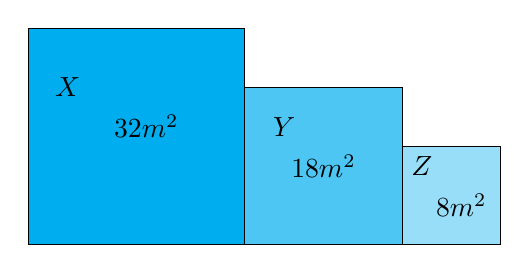
\begin{tikzpicture}[scale=.5]
	\draw[fill=cyan,very thin] (0,0) rectangle (5.5,5.5);
	\draw[fill=cyan!70, very thin] (5.5,0) rectangle (9.5,4);
	\draw[fill=cyan!40, very thin] (9.5,0) rectangle (12,2.5);
	\draw (1,4) node{$X$};
	\draw (3,3) node{$32 m^2$};
	\draw (6.5,3) node{$Y$};
	\draw (7.5,2) node{$18 m^2$};
	\draw (10,2) node{$Z$};
	\draw (11,1) node{$8 m^2$};
	\draw[thin] (0,0)--(0,5.5)--(5.5,5.5)--(5.5,4)--(9.5,4)--(9.5,2.5)--(12,2.5)--(12,0)--(0,0);
	\end{tikzpicture}
	\end{center}
	\loigiai{
	Độ dài một cạnh của thửa ruộng $X$ là: $\sqrt{32} = 4\sqrt{2}$ (m).\\
	Độ dài một cạnh của thửa ruộng $Y$ là: $\sqrt{18}=3\sqrt{2}$ (m).\\
	Độ dài một cạnh của thửa ruộng $Z$ là: $\sqrt{8} = 2\sqrt{2}$ (m).\\
	Chu vi của vườn hoa là: $4(4\sqrt{2} + 3\sqrt{2}+2\sqrt{2}) - 2(3\sqrt{2} + 2\sqrt{2}) = 26\sqrt{2}$ (m).
	}
\end{bt}
%%==========Bài 15
\begin{bt}
	Tam giác $ABC$ được vẽ trên lưới ô vuông như hình dưới. Tính diện tích và chu vi tam giác $ABC$.
	\begin{center}
	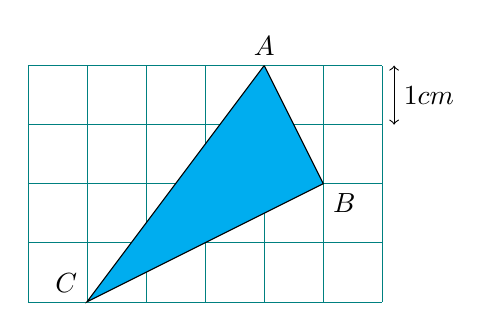
\begin{tikzpicture}[scale=.75]
	\draw[step=1,teal,very thin] (0,0) grid (6,4);
	\draw[fill=cyan] (4,4) node[above]{$A$}--(1,0) node[above left]{$C$}--(5,2) node[below right]{$B$}--(4,4);
	\draw[<->] (6.2,4)--(6.2,3.5) node[right]{$1 cm$}--(6.2,3);
	\end{tikzpicture}
	\end{center}
	\loigiai{
	Độ dài cạnh $AB=\sqrt{2^2+1^2} = \sqrt{5} $ (cm).\\
	Độ dài cạnh $AC=\sqrt{3^2 + 4^2}=\sqrt{25} = 5 $ (cm).\\
	Độ dài cạnh $BC=\sqrt{4^2 + 2^2} = \sqrt{20}=2\sqrt{5} $ (cm).\\
	Ta có $AC^2 = 5^2 =25$\\
	$AB^2 + BC^2 = (\sqrt{5})^2 + (2\sqrt{5})^2 = 25$\\
	Do đó $AC^2 = AB^2 + BC^2$\\
	Vậy tam giác $ABC$ vuông tại $B$.\\
	Diện tích tam giác $ABC$ là: $S_{ABC} = \dfrac{1}{2}\cdot AB\cdot BC = \dfrac{1}{2}\cdot \sqrt{5}\cdot 2\sqrt{5} = 5$ (cm$^2$).\\
	Chu vi tam giác $ABC$ là: $C_{ABC} = AB+AC+BC= \sqrt{5}+5+2\sqrt{5} = 5+3\sqrt{5}$ (cm).
	}
\end{bt}